%=================================================================
% 物联网学报：面向无人机遥感异构网络的注意力LSTM增强型风险感知垂直切换算法
% LaTeX 中文版（ctexart）
%=================================================================
\documentclass[10pt,a4paper]{ctexart}
\usepackage{amsmath,amssymb,booktabs,graphicx,geometry,hyperref,array,float,caption}
\geometry{left=2.0cm,right=2.0cm,top=2.7cm,bottom=2.1cm}
\graphicspath{{./plots_chapter3_v2/}}
\setmainfont{Liberation Serif}
\setsansfont{Noto Sans}
\setCJKmainfont{Noto Serif CJK SC}
\setCJKsansfont{Noto Sans CJK SC}
\setlength{\parindent}{2em}
\setlength{\parskip}{0pt}
\renewcommand{\arraystretch}{1.2}
\DeclareCaptionLabelFormat{iotjournal}{#1#2}
\captionsetup{font=small,labelformat=iotjournal,labelsep=quad}
\captionsetup[table]{position=top,justification=centering,singlelinecheck=false}
\captionsetup[figure]{justification=centering}
\newcommand{\upcite}[1]{\textsuperscript{[#1]}}
\ctexset{
  section={
    format=\heiti\zihao{4}\raggedright,
    aftername=\quad,
    beforeskip=1.0ex,
    afterskip=0.8ex
  },
  subsection={
    format=\heiti\zihao{-4}\raggedright,
    aftername=\quad,
    beforeskip=0.8ex,
    afterskip=0.5ex
  },
  subsubsection={
    format=\heiti\normalsize\raggedright,
    aftername=\quad,
    beforeskip=0.6ex,
    afterskip=0.4ex
  }
}

\title{\heiti\zihao{3} 面向无人机遥感异构网络的注意力LSTM增强型风险感知垂直切换算法}
\author{\fangsong 多滨$^{[1]}$，刘同$^{[1]}$，郑宇翔$^{[1]}$，苏文$^{[1]}$\\[2mm]
\small （1. 成都理工大学，四川省成都市 610000）}
\date{}

\begin{document}
\pagestyle{plain}
\fontsize{10.5pt}{15.75pt}\selectfont
\maketitle
\thispagestyle{plain}

\noindent{\heiti 摘\quad 要：}{\songti 无人机遥感监测系统在灾害评估、环境监测等大范围对地观测场景中广泛应用。无人机巡航时需持续穿越5G、LTE和WiFi三种异构网络的覆盖边界，构成典型的候选网络垂直切换场景，面临决策滞后、乒乓切换频繁以及固定属性权重难以适应动态飞行阶段的挑战。该研究提出了一种基于长短期记忆网络与注意力机制的自适应垂直切换方法（Long Short-Term Memory-Attention based Adaptive Vertical Handover Algorithm，LAAVHA），并在其基础上引入自适应滞后（Adaptive Dynamic Hysteresis，ADH）与风险敏感TOPSIS（Risk-Sensitive TOPSIS，RS-TOPSIS）两项增强机制，形成增强型风险感知垂直切换算法（Attention-LSTM Enhanced Risk-aware Vertical Handoff Algorithm，ALERA）。该方法利用堆叠LSTM预测候选网络短期状态变化，通过注意力机制根据飞行阶段和移动状态动态生成属性权重，融合当前状态与预测状态来构建改进的逼近理想解排序法（Technique for Order Preference by Similarity to Ideal Solution，TOPSIS）决策矩阵；以TOPSIS贴近度评分优势阈值和连续确认窗口构成双重滞后机制，抑制不必要切换。增强机制进一步采用ADH依据飞行速度和信道波动自适应调节上述阈值与确认窗口，并以RS-TOPSIS对候选网络评分施加波动风险惩罚，提升信道剧烈波动场景下的决策鲁棒性。大量仿真实验表明，所提算法可减少无效切换、提高切换决策效率并保障遥感数据回传连续性，在信道突变条件下具有更强的抗扰能力。}\\[3mm]
\noindent{\heiti 关键词：}{\songti 无人机遥感；异构网络；垂直切换；LSTM；注意力机制；自适应滞后；风险敏感TOPSIS}\\[4mm]

\begin{center}
{\bfseries Attention-LSTM Enhanced Risk-aware Vertical Handoff Algorithm for UAV Remote Sensing Heterogeneous Networks}\\[1mm]
DUO Bin$^{[1]}$, LIU Tong$^{[1]}$, ZHENG Yuxiang$^{[1]}$, SU Wen$^{[1]}$\\[1mm]
{\small 1. Chengdu University of Technology, Chengdu 610000, China}
\end{center}
\noindent{\bfseries Abstract:} Unmanned aerial vehicle (UAV) remote sensing systems are widely used in large-area earth observation scenarios such as disaster assessment and environmental monitoring. During cruise missions, UAVs continuously traverse the coverage boundaries of three heterogeneous networks---5G, LTE, and WiFi---forming a typical candidate-network vertical handover scenario that faces decision delay, frequent ping-pong handovers, and the inability of fixed attribute weights to adapt to dynamic flight phases. This study proposes an adaptive vertical handover method based on long short-term memory and an attention mechanism (Long Short-Term Memory-Attention based Adaptive Vertical Handover Algorithm, LAAVHA). On this basis, two enhancement mechanisms, adaptive dynamic hysteresis (Adaptive Dynamic Hysteresis, ADH) and risk-sensitive TOPSIS (Risk-Sensitive TOPSIS, RS-TOPSIS), are introduced to form an enhanced risk-aware vertical handoff algorithm (Attention-LSTM Enhanced Risk-aware Vertical Handoff Algorithm, ALERA). The proposed method uses a stacked LSTM to predict short-term changes in candidate-network states and an attention mechanism to generate dynamic attribute weights according to the flight phase and mobility state. Current and predicted states are fused to construct an improved Technique for Order Preference by Similarity to Ideal Solution (TOPSIS) decision matrix. A dual hysteresis mechanism, consisting of a TOPSIS closeness-score advantage threshold and a consecutive-confirmation window, suppresses unnecessary handovers. ADH further adjusts the threshold and confirmation window according to flight speed and channel fluctuations, while RS-TOPSIS applies a volatility-risk penalty to candidate-network scores, thereby improving decision robustness under severe channel fluctuations. Extensive simulations show that the proposed algorithm reduces unnecessary handovers, improves handover-decision efficiency, maintains the continuity of remote sensing data transmission, and provides stronger resistance to abrupt channel changes.\\[2mm]
\noindent{\bfseries Key words:} UAV remote sensing, heterogeneous network, vertical handover, LSTM, attention mechanism, adaptive hysteresis, risk-sensitive TOPSIS

\setcounter{section}{-1}
\section{引言}

无人机遥感系统在灾害评估、农业普查、环境监测等领域广泛应用，无人机搭载的高分辨率光学/多光谱载荷在巡航过程中产生大量遥感图像数据，需通过5G、LTE和WiFi等异构无线网络实时回传至地面站\upcite{1--3}。然而，无人机的高机动性导致其频繁穿越不同网络的覆盖边界，触发垂直切换\upcite{4}。传统垂直切换研究主要围绕多属性决策方法展开，如TOPSIS\upcite{7--8}、VIKOR\upcite{22}、GRA\upcite{22}、COPRAS\upcite{22}、SPOTIS\upcite{22}、Fuzzy-VHO\upcite{4}和SAW等，通过构建信噪比、时延、吞吐量等网络属性的评价矩阵进行候选排序。这些方法存在两个共性问题：一是权重通常由熵权法或层次分析法一次性确定\upcite{10--11}，无法随飞行阶段和信道环境动态调整；二是仅依据当前时刻的网络指标做决策，缺乏对未来状态变化的前瞻性判断，例如，当无人机高速飞向WiFi覆盖边缘时，可能在链路实际中断后才触发切换\upcite{12--13}。此外，近年深度强化学习（DRL）方法被引入切换决策\upcite{12--14}，但其黑箱性质和训练不稳定性在安全攸关的遥感巡航场景中带来可解释性和可靠性方面的顾虑。

长短期记忆网络（LSTM）通过门控结构有效缓解梯度消失问题\upcite{15}，具有捕获长时间序列依赖关系的能力，已被应用于5G异构网络的切换判决和网络状态预测\upcite{16--17}。然而，单一LSTM网络存在两方面局限：其一，LSTM将候选网络的5维状态指标视为独立的时间序列分别建模，无法显式捕获指标之间的耦合关系，例如吞吐量与丢包率的负相关性、SINR与时延的关联性等；其二，LSTM输出的预测状态仍需配合固定或人工设定的属性权重才能完成多属性决策，无法根据飞行阶段和移动状态自适应调整各指标的重要性。

综上所述，当前无人机遥感异构网络中的垂直切换面临两个层面的挑战：在算法层面，传统多属性决策方法（Multiple Attribute Decision Making, MADM）权重固定、缺乏时序预测能力，单一LSTM即使引入预测机制仍无法自适应调节属性权重以适应飞行阶段变化；在场景层面，无人机巡航过程中信道环境动态变化：平稳飞行时信号波动小，跨越覆盖边界或遭遇遮挡时信号剧烈振荡，固定的切换阈值和确认窗口难以在两者之间取得平衡。两个层面的问题相互关联：算法适应性的不足加剧了场景波动带来的切换不稳定，而场景的动态变化又要求算法具备更强的环境感知能力。

针对上述两个层面相互关联的挑战，本文提出分层次的解决方案。在算法层面，构建基于长短期记忆神经网络和注意力机制的自适应垂直切换算法（LAAVHA），以引入注意力机制弥补传统MADM方法在动态权重与时序预测方面的不足。LAAVHA采用预测、权重与决策三阶段架构：堆叠LSTM预测候选网络短期状态变化；注意力机制以当前网络状态矩阵为自注意力输入，融合飞行速度与高度等移动特征，输出随飞行阶段自适应变化的动态属性权重；融合当前与预测状态构建改进TOPSIS决策矩阵，并以TOPSIS贴近度评分优势阈值和连续确认窗口组成的双重滞后机制完成候选排序与切换裁定。LAAVHA通过动态权重与前瞻预测，克服了传统MADM方法权重固定和被动响应的问题，实现了无人机遥感巡航场景下的稳定候选网络评价。在场景层面，无人机遥感探测任务具有广域巡航、高速跨越5G/LTE/WiFi覆盖边界以及跨越边界或遭遇遮挡时信道突变等特点；同时，高分辨率遥感图像需要在飞行过程中持续、可靠地回传。为满足这一场景需求，在LAAVHA决策框架之上进一步引入自适应滞后（ADH）与风险敏感TOPSIS（RS-TOPSIS）两项增强机制，形成注意力LSTM增强型风险感知垂直切换算法（ALERA）。ADH将固定的切换阈值与确认窗口替换为上下文感知的可变参数：以服务网络近5个周期的SINR标准差度量信道波动，阈值随波动从0.03线性增长至0.08，确认窗口随飞行速度在$[2,4]$范围内自适应缩短（此参数取值依据会在后续实验进行说明）。RS-TOPSIS依据候选网络近期TOPSIS贴近度评分的波动程度施加风险罚分：评分越不稳定，排序时扣减越大，从而优先选择历史表现更稳定的网络。两项增强机制不改变LSTM与注意力网络的模型结构和训练过程，而是在候选网络评分生成之后、最终执行切换之前的规则判定环节发挥作用：ADH调整切换阈值与确认窗口，RS-TOPSIS调整候选网络的排序依据，二者协同实现信道波动感知与风险规避决策，使算法更适配遥感探测场景下的持续可靠回传需求。

\section{网络场景与网络状态参数}

考虑无人机遥感巡航场景：无人机在$2000~\mathrm{m}\times2000~\mathrm{m}$的任务区域内沿预定航线飞行，飞行高度为$50\sim150~\mathrm{m}$，巡航速度为$5\sim30~\mathrm{m/s}$。任务区域内存在WiFi、LTE和5G三种候选接入网络，其覆盖范围与部署密度各不相同：WiFi热点覆盖半径约$200~\mathrm{m}$，部署于地面站和关键拍摄点周边；LTE基站覆盖半径约$1\sim2~\mathrm{km}$，沿航线稀疏分布；5G基站覆盖半径约$500~\mathrm{m}$，部署于任务区域东侧的遥感数据汇聚位置，提供高速率接入但覆盖尚不连续。无人机在飞行过程中周期性采集各候选网络的状态信息，用于切换决策\upcite{21}。

\begin{figure}[H]
\centering
\caption{无人机遥感任务区域中的异构网络覆盖与移动轨迹示意}
\label{fig:network_coverage}
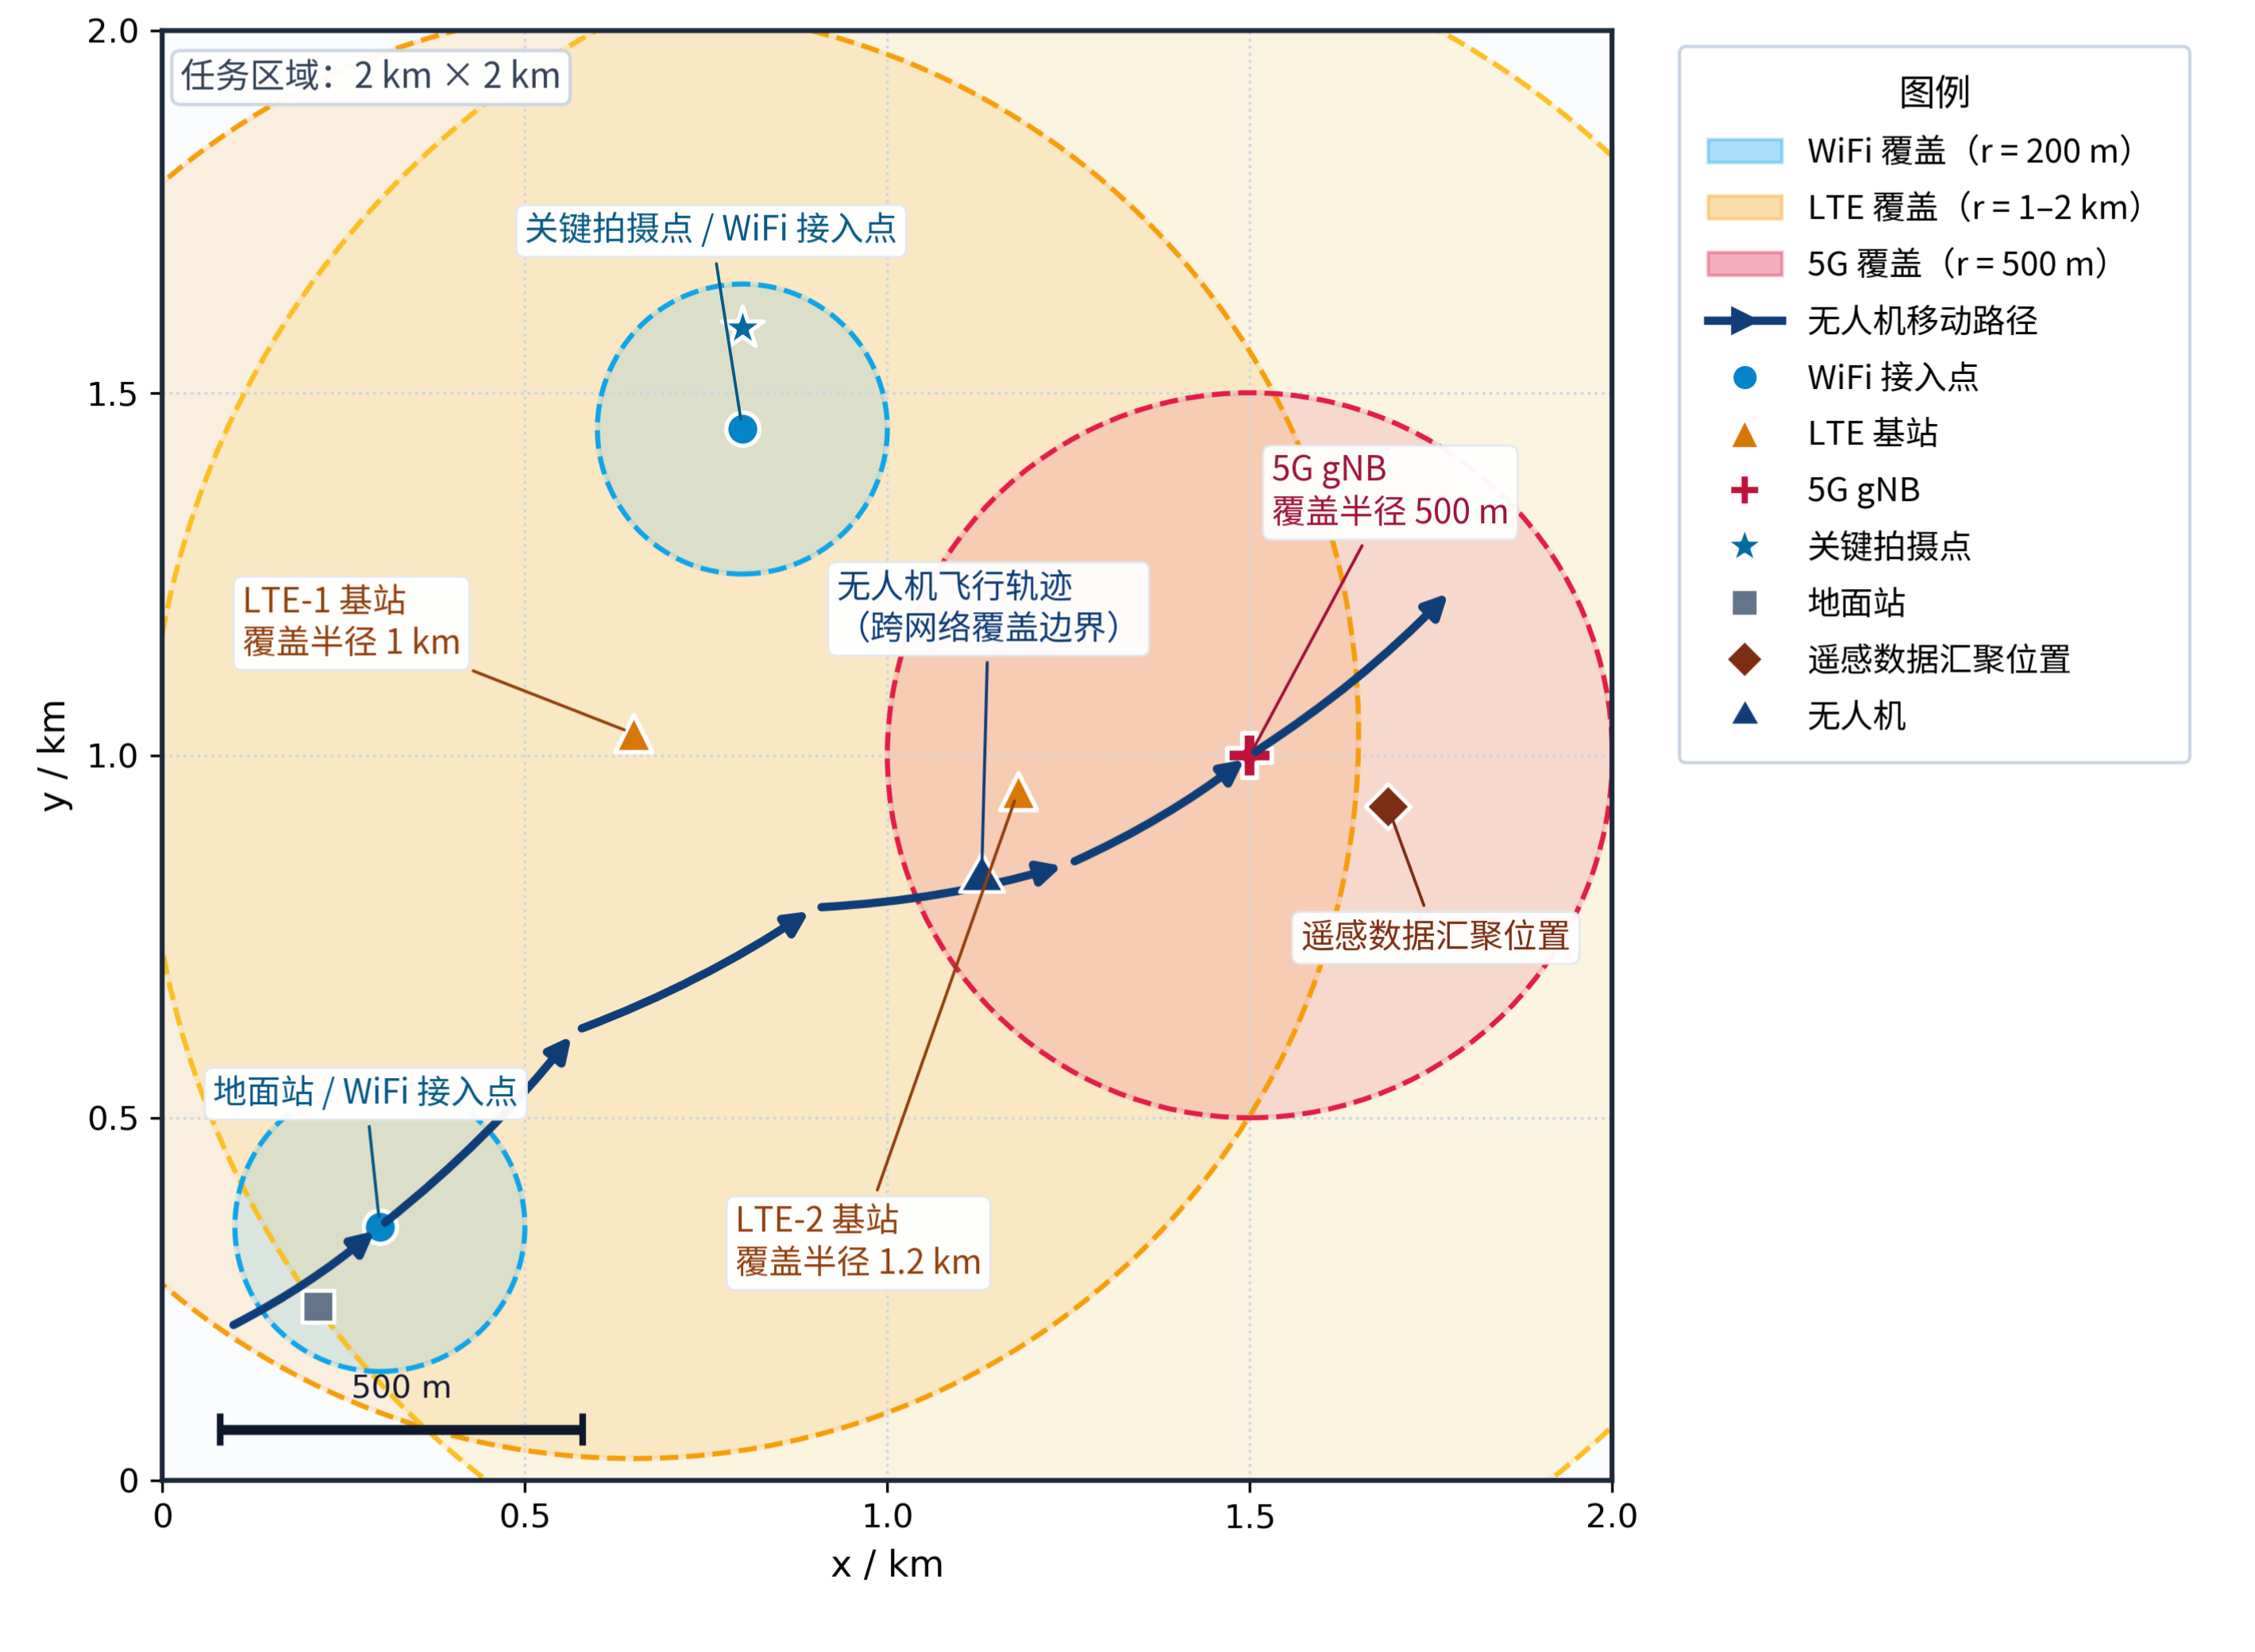
\includegraphics[width=\textwidth]{plots_chapter3_v2.png}
\end{figure}

如图\ref{fig:network_coverage}所示，任务区域内三类网络形成尺度不同且相互重叠的覆盖空间：WiFi热点覆盖范围较小，主要服务地面站和关键拍摄点附近的数据接入；LTE基站覆盖范围较广，为无人机广域巡航提供连续性较强的基础连接；5G基站部署于任务区域东侧的数据汇聚位置，在有限覆盖范围内提供高速率传输。图中的5G gNB（next generation NodeB）表示5G无线接入基站，负责为无人机提供5G信号覆盖、无线资源调度和高速数据传输服务。无人机沿预定轨迹飞行时依次进入、离开并穿越不同网络的重叠覆盖区域，当当前服务网络质量下降而其他候选网络的综合性能上升时，需要执行垂直切换。图中各覆盖圆的相对尺度与前述覆盖半径设置一致，为后续网络状态采集和候选网络评价提供场景基础。

对于第$i$个候选网络，其在时刻$t$的状态向量定义为
\begin{equation}
S_i(t)=\left[\mathrm{SINR}_i(t),\,\mathrm{RSRP}_i(t),\,D_i(t),\,T_i(t),\,\mathrm{PLR}_i(t)\right].
\label{eq:state}
\end{equation}

在遥感飞行场景中，上述五个指标从不同维度刻画了候选网络服务遥感任务的能力：当无人机从WiFi热点上空飞向任务区域边缘时，信噪比$\mathrm{SINR}_i(t)$从数十dB单调下降至接近噪声底限，直接反映了信号质量随距离和遮挡的衰减过程，是判断是否触发切换的最直观依据；参考信号接收功率$\mathrm{RSRP}_i(t)$与$\mathrm{SINR}_i(t)$共同决定链路预算是否满足解调门限；若$\mathrm{RSRP}_i(t)$低于接收灵敏度，即使$\mathrm{SINR}_i(t)$尚可，物理层也无法建立可靠连接；端到端时延$D_i(t)$定义为数据包从地面站到达无人机应用层的往返时间，在高速巡航阶段直接决定飞控指令的响应速度与飞行安全冗余度；吞吐量$T_i(t)$衡量候选网络单位时间内可交付的有效载荷比特数，对单张可达数MB的高分辨率遥感图像而言，$T_i(t)$不足将导致单次过顶时间内无法完成图像下传；丢包率$\mathrm{PLR}_i(t)$反映网络传输的可靠性，即使在信号较强、吞吐量充裕的位置，较高的$\mathrm{PLR}_i(t)$也会使接收端重建的遥感图像出现条带缺失或块状模糊。上述指标中，$\mathrm{SINR}_i(t)$、$\mathrm{RSRP}_i(t)$和$T_i(t)$属于效益型指标（数值越大越优），$D_i(t)$和$\mathrm{PLR}_i(t)$属于成本型指标（数值越小越优）。为消除各指标量纲差异，采用min-max归一化方法将所有指标映射至$[0,1]$区间，并使归一化后的值越大表示候选网络在该维度上越优\upcite{22}。

因此，式\eqref{eq:state}不是单独用于描述网络状态的静态定义，而是后续算法链路的统一输入接口。对同一时刻3个候选网络的$S_i(t)$按网络维度堆叠，可得到当前状态矩阵$S_{\mathrm{cur}}\in\mathbf{R}^{3\times5}$，该矩阵直接输入第2.2节的注意力权重生成模块；对单个候选网络连续10个决策周期的状态向量按时间维度堆叠，可得到历史状态张量$X_k\in\mathbf{R}^{10\times5}$，该张量输入第2.1节的堆叠LSTM预测模块。也就是说，第1章给出的网络状态参数同时承担两类作用：横向上刻画同一时刻不同候选网络的优劣差异，纵向上刻画同一网络随无人机运动产生的短期演化趋势。

无人节点移动会引起候选网络信号质量和传输性能持续变化。在遥感巡航场景中，若仅依据当前时刻指标进行切换决策，无人机可能在高速接近WiFi覆盖边缘时未能提前切换，导致正在回传的图像数据因链路突然中断而丢失\upcite{23}。因此，算法将过去若干个决策周期的网络状态组织为时序输入，用于预测短期未来状态，并将预测结果与当前状态共同用于最终决策。

\section{LAAVHA自适应垂直切换算法}

基于第1章定义的网络场景与网络状态参数，本章提出基于长短期记忆神经网络和注意力机制的自适应垂直切换算法（LAAVHA），旨在解决传统MADM方法在无人机遥感巡航场景中权重固定和缺乏时序预测能力的不足。LAAVHA以第1章所述的5维网络状态向量和滑动窗口机制为输入，依次通过堆叠LSTM预测、注意力动态权重生成和融合预测状态的改进TOPSIS决策三个模块完成候选网络评估与切换判决，最后引入自适应滞后（ADH）与风险敏感TOPSIS（RS-TOPSIS）两项增强机制形成ALERA。

\begin{figure}[H]
\centering
\caption{LAAVHA与ALERA算法框架}
\label{fig:frameworks}
(a) LAAVHA算法框架\\[1mm]
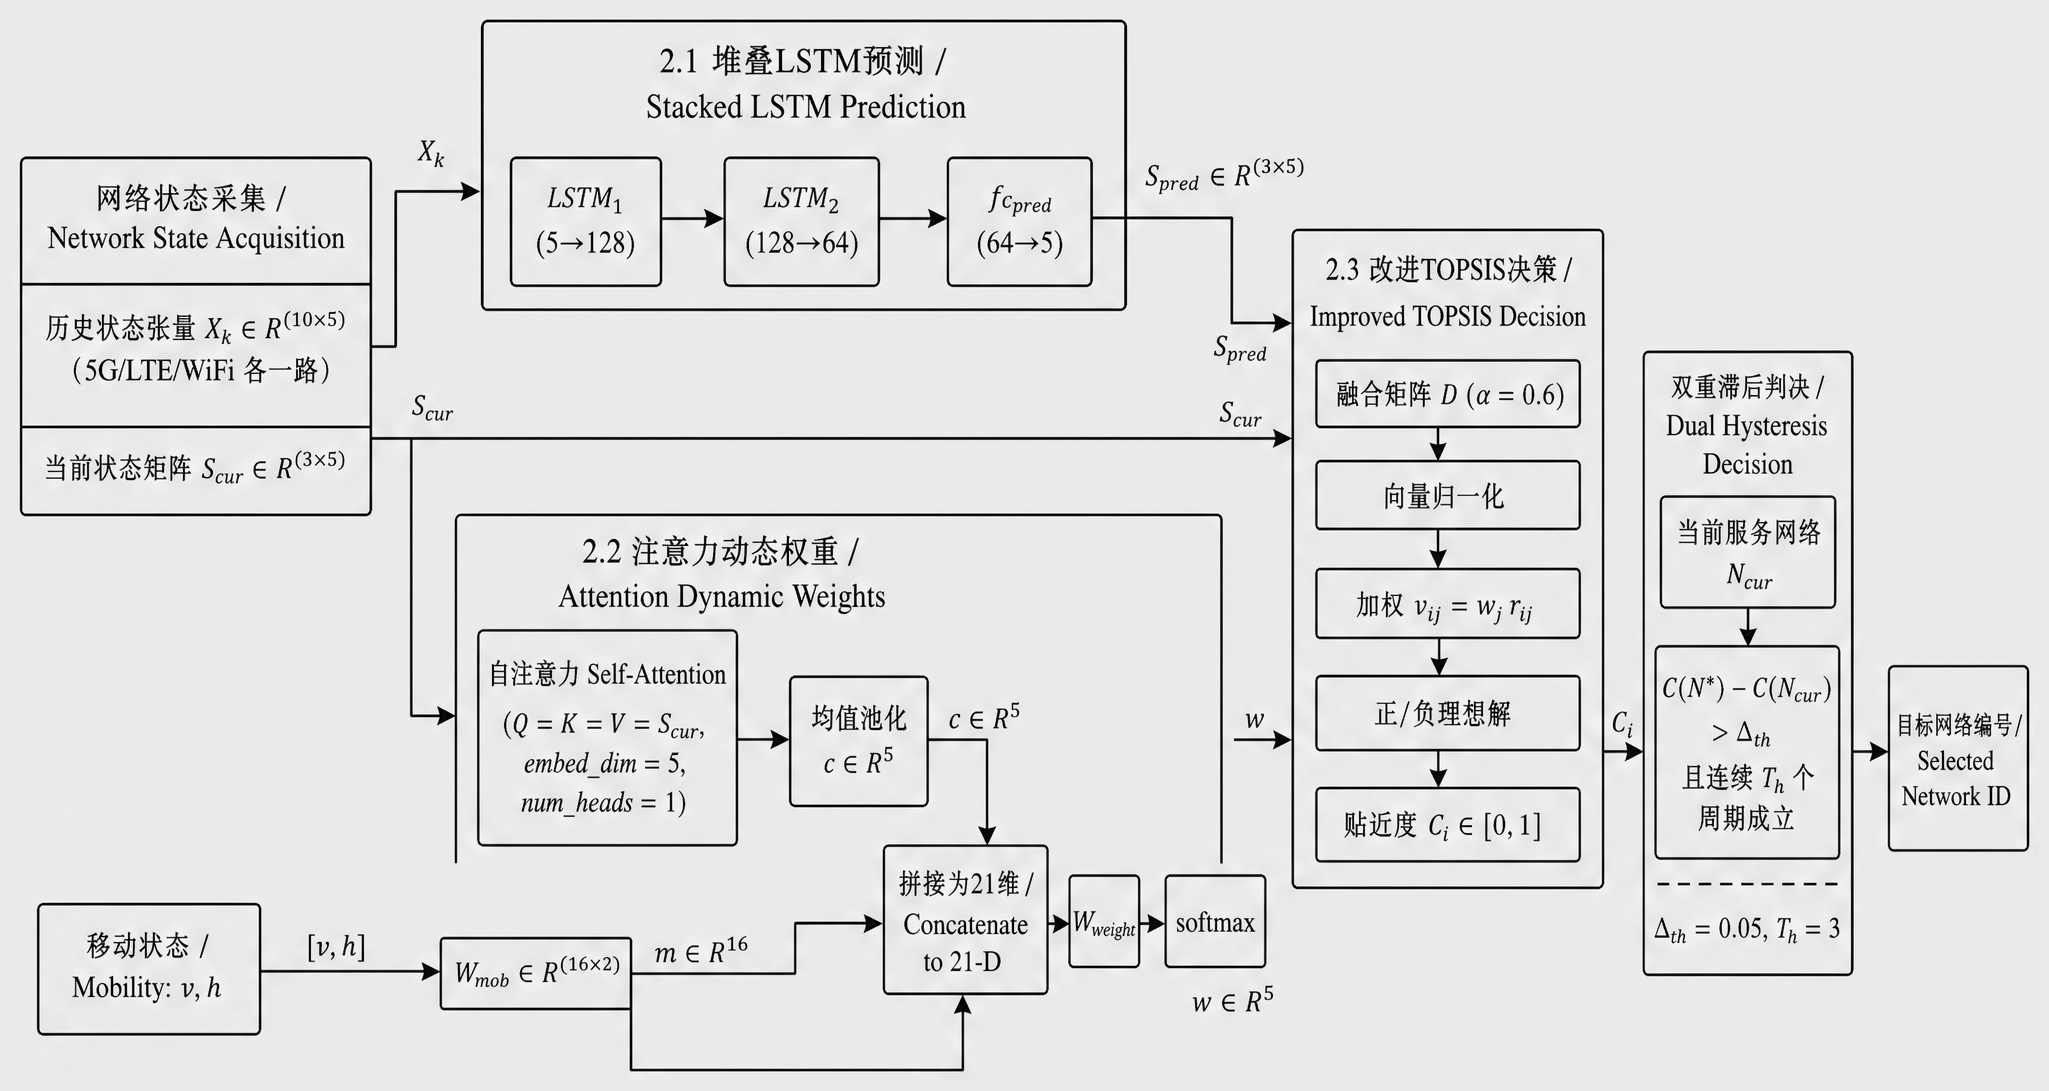
\includegraphics[width=\textwidth]{fig_laavha_framework_v3.png}\\[3mm]
(b) ALERA算法框架\\[1mm]
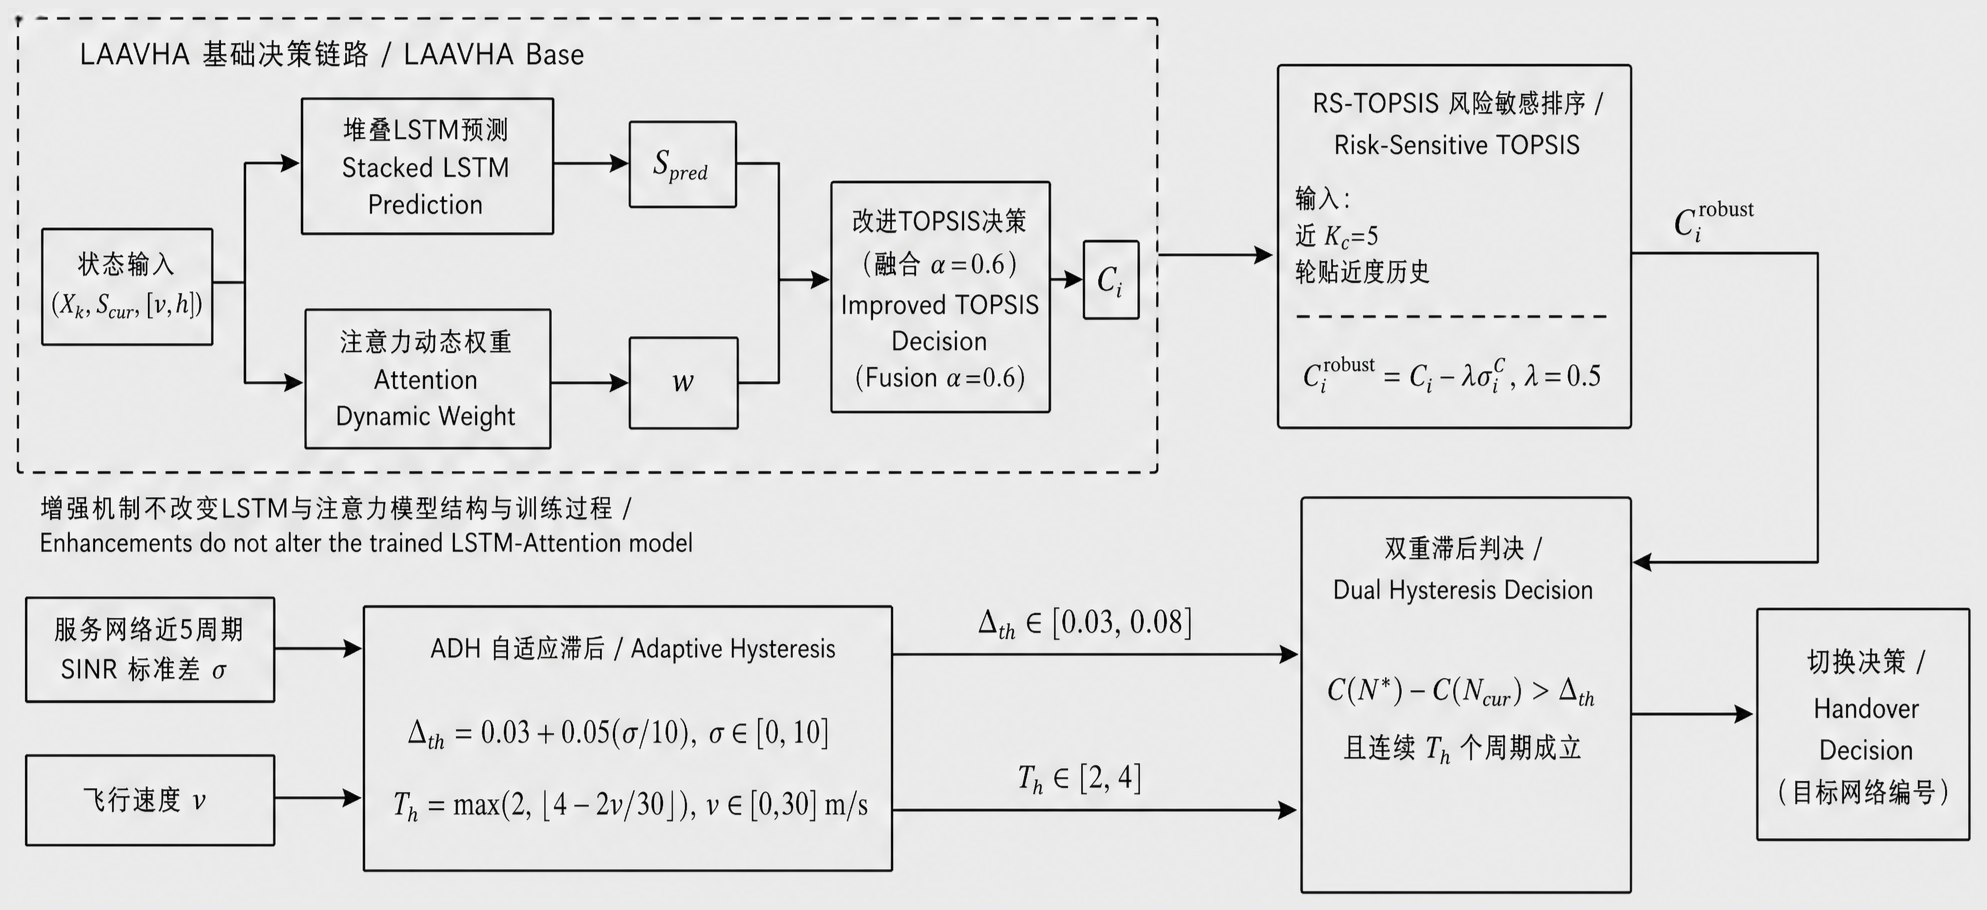
\includegraphics[width=\textwidth]{fig_alera_framework_v3.png}
\end{figure}

图\ref{fig:frameworks}中的各模块并非并列孤立运行，而是围绕同一组网络状态形成端到端变量流：由第1章采集并归一化后的历史序列$X_k$首先进入堆叠LSTM，得到下一时刻预测状态$S_{\mathrm{pred}}$；同一决策周期的当前状态矩阵$S_{\mathrm{cur}}$进入注意力模块，与速度、高度等移动特征共同生成动态权重$w$；随后$S_{\mathrm{cur}}$、$S_{\mathrm{pred}}$和$w$在改进TOPSIS模块中汇合，输出候选网络贴近度$C_i$；最后，$C_i$与当前接入网络$N_{\mathrm{cur}}$共同进入滞后判决和ALERA增强机制，形成最终切换决策。按照这一链路，2.1节解决``未来状态是什么''，2.2节解决``当前任务更重视哪些指标''，2.3节解决``综合当前与未来后哪个网络更优''，2.4节进一步解决``在波动环境下是否应该执行这次切换''。

\subsection{基于堆叠LSTM的网络状态预测}

设时间窗口长度$T_s=10$（即覆盖$1.0~\mathrm{s}$内的10个连续决策周期，决策周期$\tau=0.1~\mathrm{s}$），候选网络$k\in\{1,2,3\}$（分别对应5G、LTE、WiFi）的历史输入张量为$X_k\in\mathbf{R}^{10\times5}$，其中10个连续决策周期的5维归一化状态向量按行堆叠。预测目标是下一时刻的状态向量$\hat{s}_k(t+\tau)\in\mathbf{R}^5$。
\begin{align}
h_{1,k} &= \mathrm{LSTM}_1(X_k;\theta_1), && h_{1,k}\in\mathbf{R}^{10\times128}, \label{eq:lstm1}\\
h_{2,k} &= \mathrm{LSTM}_2(h_{1,k};\theta_2), && h_{2,k}\in\mathbf{R}^{10\times64}, \label{eq:lstm2}\\
\hat{s}_k(t+\tau) &= W_{\mathrm{pred}}h_{2,k}[-1]+b_{\mathrm{pred}}, && \hat{s}_k\in\mathbf{R}^5. \label{eq:lstm3}
\end{align}
式中$\theta_1$、$\theta_2$分别为两层LSTM的可训练参数（含输入门、遗忘门、输出门及细胞状态的权重与偏置），$W_{\mathrm{pred}}\in\mathbf{R}^{5\times64}$与$b_{\mathrm{pred}}\in\mathbf{R}^5$为预测头的全连接权重与偏置，$h_{2,k}[-1]$表示取$\mathrm{LSTM}_2$最后时刻的输出向量。式\eqref{eq:lstm1}至式\eqref{eq:lstm3}完整刻画了预测分支的维度变换：10步$\times$5维指标$\rightarrow\mathrm{LSTM}_1(5\rightarrow128)\rightarrow\mathrm{LSTM}_2(128\rightarrow64)\rightarrow$fc\_pred($64\rightarrow5$)。三个候选网络共享同一组LSTM参数（即对5G、LTE、WiFi使用相同的$\theta_1$、$\theta_2$、$W_{\mathrm{pred}}$、$b_{\mathrm{pred}}$），各自独立输入历史序列$X_k$，预测结果堆叠为$S_{\mathrm{pred}}\in\mathbf{R}^{3\times5}$，即三个网络各自下一时刻的五项指标预测值。

需要强调的是，$S_{\mathrm{pred}}$并不是直接决定切换目标的最终评分，而是把历史序列$X_k$压缩为下一决策周期可比较的预测状态。其作用是在第2.3节式\eqref{eq:fuse}中与当前状态$S_{\mathrm{cur}}$共同构成融合决策矩阵，使TOPSIS排序同时具有当前实测依据和短期前瞻信息。若没有这一输出，后续决策只能退化为对$S_{\mathrm{cur}}$的被动排序，这正是消融变体LAAVHA-L用于检验的部分。

\subsection{面向飞行阶段的动态权重生成}

在垂直切换决策中，不同网络属性的重要性会随场景变化而变化。例如，无人机处于巡航飞行阶段时，链路稳定性和控制指令时延对飞行安全更加关键；当抵达拍摄点进入图像回传阶段时，吞吐量和丢包率的权重应显著提升，以确保高分辨率遥感图像在有限时间窗口内完整送达地面站\upcite{24}。固定权重难以刻画这种动态变化。

为解决固定权重无法匹配遥感飞行中不同阶段需求差异的问题，LAAVHA引入自注意力机制（Self-Attention）\upcite{18}。将当前3个候选网络的5维状态向量按行堆叠为矩阵$S_{\mathrm{cur}}\in\mathbf{R}^{3\times5}$，令自注意力的查询（Query）、键（Key）、值（Value）均等于$S_{\mathrm{cur}}$（即$Q=K=V=S_{\mathrm{cur}}$，\texttt{embed\_dim}=5, \texttt{num\_heads}=1）。其中，\texttt{embed\_dim}表示注意力模块中每个输入向量的特征维度；本文每个候选网络由SINR、RSRP、时延、吞吐量和丢包率5个归一化指标描述，因此\texttt{embed\_dim}取5，与$S_{\mathrm{cur}}$的列数一致。\texttt{num\_heads}表示并行注意力头的数量；由于本文属性维度仅为5，若采用多头注意力会使每个头分到的特征维度过小，不利于解释各指标权重，因此采用单头注意力（\texttt{num\_heads}=1）直接学习5个属性之间的相关性。随后通过缩放点积注意力计算属性间的交互权重，其中注意力矩阵$A$的每个元素$a_{ij}$表示属性$j$对属性$i$的重要性。再经跨网络均值池化提取属性级上下文$c\in\mathbf{R}^5$，并联飞行速度$v$与高度$h$经$W_{\mathrm{mob}}\in\mathbf{R}^{16\times2}$映射为移动特征$m\in\mathbf{R}^{16}$，拼接后经全连接层投影与softmax归一化输出5维动态权重$w$：
\begin{align}
Q &= K = V = S_{\mathrm{cur}}\in\mathbf{R}^{3\times5}, \label{eq:attn1}\\
A &= \mathrm{Attention}(Q,K,V)=\mathrm{softmax}\!\left(\frac{QK^\top}{\sqrt{5}}\right)V,\quad A\in\mathbf{R}^{3\times5}, \label{eq:attn2}\\
c &= \mathrm{mean}(A,\mathrm{dim}=0)\in\mathbf{R}^5, \label{eq:attn3}\\
m &= \mathrm{ReLU}\!\left(W_{\mathrm{mob}}[v,h]^\top\right),\quad W_{\mathrm{mob}}:\mathbf{R}^{2}\rightarrow\mathbf{R}^{16},\quad m\in\mathbf{R}^{16}, \label{eq:attn4}\\
w &= \mathrm{softmax}\!\left(W_{\mathrm{weight}}[c\parallel m]\right),\quad W_{\mathrm{weight}}:\mathbf{R}^{21}\rightarrow\mathbf{R}^{5},\quad w\in\mathbf{R}^{5},\quad \sum_j w_j=1. \label{eq:attn5}
\end{align}
式\eqref{eq:attn1}至式\eqref{eq:attn5}描述了动态权重的完整生成过程：以当前时刻网络状态$S_{\mathrm{cur}}\in\mathbf{R}^{3\times5}$为自注意力输入，缩放点积注意力获得$3\times5$注意力矩阵$A$；跨网络均值池化得到5维属性级上下文$c$；$W_{\mathrm{mob}}:2\rightarrow16$将速度和高度映射为16维移动特征$m$引入飞行状态；最后拼接为21维经$W_{\mathrm{weight}}$投影和softmax归一化输出5维动态权重$w$。

因此，注意力模块的输出$w$也不是单独评价网络优劣的结果，而是第2.3节TOPSIS加权步骤的输入。具体而言，式\eqref{eq:topsis2}中的$v_{ij}=w_j r_{ij}$将$w_j$作用到融合矩阵$D$的第$j$个属性维度，使SINR、RSRP、时延、吞吐量和丢包率的相对重要性能够随当前网络状态和飞行状态变化。这样，LSTM分支提供``预测到哪里去''，Attention分支提供``当前该重视什么''，二者在TOPSIS排序阶段共同影响最终贴近度$C_i$。

\subsection{融合预测状态的改进TOPSIS决策}

本节是前述两个学习模块的汇合点：第2.1节输出的$S_{\mathrm{pred}}$提供短期未来状态，第2.2节输出的$w$提供当前飞行阶段下的属性重要性，第1章定义并实时采集的$S_{\mathrm{cur}}$提供当前观测状态。在遥感巡航场景中，候选网络的优劣需要综合权衡信号强度、传输能力与可靠性三个维度，不存在单一指标最优的``完美网络''。TOPSIS的基本思想是将各候选网络在多维属性空间中的位置与虚拟的``最优网络''和``最劣网络''进行比较\upcite{7--8}。为避免传统TOPSIS仅依赖当前状态导致的被动决策，LAAVHA首先将当前状态与LSTM预测状态进行融合，构建决策矩阵：
\begin{align}
s_{\mathrm{norm}} &= \frac{s-s_{\min}}{s_{\max}-s_{\min}},\quad \text{for each indicator }j, \label{eq:norm}\\
d_{ij} &= \alpha s_{\mathrm{cur}}(i,j)+(1-\alpha)s_{\mathrm{pred}}(i,j),\quad \alpha=0.6, \label{eq:fuse}\\
d_{ij} &\leftarrow 1-d_{ij},\quad j\in\{\mathrm{delay},\mathrm{PLR}\}. \label{eq:cost}
\end{align}
式\eqref{eq:norm}至式\eqref{eq:cost}中，$i$表示候选网络编号，$i=1,2,3$分别对应5G、LTE和WiFi；$j$表示属性指标编号，本文共有5个属性，即SINR、RSRP、时延、吞吐量和丢包率。$s$表示某一候选网络在第$j$个属性上的原始或待归一化指标值，$s_{\min}$和$s_{\max}$分别表示当前决策周期内该属性在全部候选网络中的最小值和最大值，$s_{\mathrm{norm}}$为映射到$[0,1]$区间后的归一化值。$s_{\mathrm{cur}}(i,j)$表示候选网络$i$在当前时刻第$j$个属性上的归一化状态值，$s_{\mathrm{pred}}(i,j)$表示LSTM预测得到的下一时刻对应属性值，$d_{ij}$表示二者融合后写入决策矩阵$D$的元素。$\alpha$为当前状态与预测状态的融合系数，本文取$\alpha=0.6$，该取值使当前实测状态占主导，同时保留预测信息的前瞻引导作用（此参数取值依据会在后续实验进行说明）。由于时延和丢包率属于成本型指标，数值越小越优，因此式\eqref{eq:cost}对其归一化值执行取反，使所有属性在进入TOPSIS前统一为``数值越大越优''。将成本型指标取反后得到融合决策矩阵$D\in\mathbf{R}^{3\times5}$，进入标准化TOPSIS流程：
\begin{align}
r_{ij} &= \frac{d_{ij}}{\sqrt{\sum_{k=1}^{3}d_{kj}^{2}}}, \label{eq:topsis1}\\
v_{ij} &= w_j r_{ij}, \label{eq:topsis2}\\
v_j^+ &= \max_i v_{ij},\quad v_j^-=\min_i v_{ij}, \label{eq:topsis3}\\
D_i^+ &= \sqrt{\sum_{j=1}^{5}(v_{ij}-v_j^+)^2},\quad
D_i^-=\sqrt{\sum_{j=1}^{5}(v_{ij}-v_j^-)^2}, \label{eq:topsis4}\\
C_i &= \frac{D_i^-}{D_i^+ + D_i^-},\quad C_i\in[0,1]. \label{eq:topsis5}
\end{align}
式\eqref{eq:topsis1}至式\eqref{eq:topsis5}中，$r_{ij}$表示融合决策矩阵$D$经向量归一化后的元素，分母$\sqrt{\sum_{k=1}^{3}d_{kj}^{2}}$为第$j$个属性在3个候选网络上的欧氏范数；此处$k$仅为求和索引，表示候选网络编号，不再表示第2.1节中的历史输入序列编号。$w_j$为第2.2节Attention模块输出的第$j$个属性动态权重，$v_{ij}$为归一化元素$r_{ij}$经权重$w_j$加权后的结果。$v_j^+$和$v_j^-$分别表示第$j$个属性上的正理想解和负理想解，即所有候选网络加权归一化值中的最大值和最小值。$D_i^+$表示候选网络$i$到正理想解的欧氏距离，$D_i^-$表示其到负理想解的欧氏距离；$C_i$为候选网络$i$的相对贴近度，取值范围为$[0,1]$。因此，式\eqref{eq:topsis1}至式\eqref{eq:topsis5}将$3\times5$的融合决策矩阵$D$转换为三个候选网络的相对贴近度排序：向量归一化消除指标量纲$\rightarrow$动态权重加权$\rightarrow$确定正/负理想解$\rightarrow$欧氏距离计算$\rightarrow$输出$C_i\in[0,1]$。$C_i$越接近1，表示该网络对遥感任务中图像回传、飞控响应和链路可靠性三者的综合保障能力越强。
\begin{align}
N^* &= \arg\max_i C_i, \label{eq:select}\\
\mathrm{Decision} &=
\begin{cases}
\text{switch to }N^*, & C(N^*)-C(N_{\mathrm{cur}})>\Delta_{\mathrm{th}}\ \text{and lasts }T_h\text{ consecutive cycles},\\
\text{keep }N_{\mathrm{cur}}, & \text{otherwise},
\end{cases} \label{eq:hysteresis}
\end{align}
式\eqref{eq:select}至式\eqref{eq:hysteresis}中，$N^*$表示当前决策周期内贴近度$C_i$最大的候选网络，$N_{\mathrm{cur}}$表示无人机当前正在接入的服务网络，$C(N^*)$和$C(N_{\mathrm{cur}})$分别表示目标候选网络和当前服务网络的TOPSIS贴近度。$\Delta_{\mathrm{th}}$为切换触发阈值，用于要求目标网络相对当前网络具有足够明显的评分优势；$T_h$为连续确认窗口，用于要求该优势连续保持若干个决策周期。本文设置$\Delta_{\mathrm{th}}=0.05$，$T_h=3$（此参数取值依据会在后续实验进行说明）。为降低网络状态瞬时波动引发的乒乓切换，算法设置双重滞后机制。式\eqref{eq:select}至式\eqref{eq:hysteresis}描述了切换的最终裁定逻辑：仅当得分最高的候选网络$N^*$的贴近度超过当前服务网络$N_{\mathrm{cur}}$达$\Delta_{\mathrm{th}}=0.05$以上，且该条件在连续$T_h=3$个决策周期内持续满足时，才正式执行切换。在遥感任务中，一次乒乓切换可能导致正在传输的图像数据包丢失。滞后机制通过阈值过滤小幅评分波动，通过时间窗口消除瞬时信道异常触发的虚假切换，两者协同保障遥感数据传输的连续性。表\ref{tab:process}是整个LAAVHA算法的总体流程，对上述预测、权重生成、TOPSIS排序和滞后裁定步骤进行汇总。

\begin{table}[H]
\centering
\caption{LAAVHA垂直切换算法总体流程}
\small
\begin{tabular}{cp{11cm}}
\toprule
步骤 & 说明 \\
\midrule
1 & 采集5G、LTE和WiFi候选网络的SINR、RSRP、时延、吞吐量和丢包率 \\
2 & 对效益型和成本型指标进行归一化处理，构建历史状态序列 \\
3 & 利用堆叠LSTM预测各候选网络短期未来状态 \\
4 & 基于注意力机制生成动态属性权重 \\
5 & 融合当前状态与预测状态，构建改进TOPSIS决策矩阵 \\
6 & 计算候选网络相对贴近度，选取得分最高的目标网络 \\
7 & 结合贴近度阈值和时间窗口滞后机制输出最终切换决策 \\
\bottomrule
\end{tabular}
\label{tab:process}
\end{table}

需要指出的是，上述TOPSIS决策流程和双重滞后机制在训练阶段用于生成监督标签：对每条历史网络状态记录，执行完整的融合决策矩阵构建、加权TOPSIS排序和滞后条件检查，将最终选定的最优网络编号作为该记录的训练目标。部署阶段，训练好的LAAVHA\_Net仅输出$S_{\mathrm{pred}}\in\mathbf{R}^{3\times5}$和$w\in\mathbf{R}^5$；神经网络不直接输出切换决策，而是作为``状态感知器''提供时序预测与动态权重；推理侧随后依次执行式\eqref{eq:fuse}的融合矩阵构建、式\eqref{eq:topsis1}至式\eqref{eq:topsis5}的TOPSIS排序和式\eqref{eq:select}至式\eqref{eq:hysteresis}的滞后裁定，最终输出目标网络编号。由此可见，$X_k$、$S_{\mathrm{cur}}$、$S_{\mathrm{pred}}$、$w$、$D$、$C_i$和$\mathrm{Decision}$构成一条连续的数据链，而不是多个互不相关的公式集合。这一``神经网络预测+规则化决策''的混合架构，使算法的每一步变换均可由式\eqref{eq:state}至式\eqref{eq:hysteresis}完整追踪，兼顾了深度学习的时序建模能力和传统多属性决策的透明性与可解释性。

\subsection{ALERA增强型风险感知垂直切换算法}

第2.3节完成了从状态预测、动态加权到候选排序和切换裁定的基础决策链路，但其中的双重滞后仍采用前述固定参数。该设置在信道平稳时表现良好，当无人机跨越覆盖边界、遭遇遮挡或飞行速度显著变化时，固定阈值与确认窗口却难以同时兼顾抗波动能力和切换时效；与此同时，原始TOPSIS仅依据当前贴近度排序，尚未对评分序列的波动风险进行约束。为承接前述基础决策并增强其遥感场景适应性，本节在不重新训练LSTM-Attention模型的条件下引入两项机制：ADH读取当前服务网络的SINR历史和飞行速度，动态更新式\eqref{eq:hysteresis}中的$\Delta_{\mathrm{th}}$与$T_h$；RS-TOPSIS读取第2.3节输出的贴近度序列$C_i$，将其修正为风险惩罚后的$C_i^{\mathrm{robust}}$再参与排序，从而形成ALERA。

\subsubsection{自适应滞后参数}

将固定阈值$\Delta_{\mathrm{th}}$和窗口$T_h$替换为上下文感知的可变参数。定义近期SINR波动度$\sigma$为当前服务网络近5个决策周期SINR的标准差，飞行速度$v$由仿真侧实时传入。这里的$\sigma$来自式\eqref{eq:state}中SINR维度的历史观测，$v$来自第2.2节已用于动态权重生成的移动状态输入，因此ADH复用已有状态信息，只改变最终滞后判决的门槛和确认长度。自适应阈值和窗口计算公式为：
\begin{align}
\Delta_{\mathrm{th}} &= 0.03+0.05\left(\frac{\sigma}{10}\right),\quad \sigma\in[0,10], \label{eq:adh1}\\
T_h &= \max\left(2,\left\lfloor4-\frac{2v}{30}\right\rfloor\right),\quad v\in[0,30]~\mathrm{m/s}. \label{eq:adh2}
\end{align}
式\eqref{eq:adh1}在信道稳定（$\sigma\approx0$）时给出基础阈值0.03，低于原始固定值0.05，为快速响应持续性链路劣化预留空间；在信道波动较为剧烈（$\sigma\approx10$）时，波动修正项使阈值线性增长至最高0.08，抬高切换门槛以抑制切换（$\sigma$的历史长度取值依据会在后续实验进行说明）。式\eqref{eq:adh2}在低速飞行（$v\approx5~\mathrm{m/s}$）时给出窗口4，提供充分的确认周期；窗口随速度增加而缩短至最低2，使高速无人机飞越覆盖边界时能及时切换。参数范围（$\Delta_{\mathrm{th}}\in[0.03,0.08]$，$T_h\in[2,4]$）确保了极端条件下的基本防抖能力（此参数取值依据会在后续实验进行说明）。窗口随速度增加而缩短的设计依据在于，无人机在高速飞行时跨越网络覆盖边界所经历的时间极短。以$30~\mathrm{m/s}$飞行时，单个决策周期（$0.1~\mathrm{s}$）内无人机已移动$3~\mathrm{m}$，若维持长窗口$T_h=4$（$0.4~\mathrm{s}$）则确认期间位移达$12~\mathrm{m}$，可能已从WiFi覆盖中心飞至边缘，初始判断在确认完成时已失效；缩短至$T_h=2$（$0.2~\mathrm{s}$，位移$6~\mathrm{m}$）使算法在覆盖边界附近能更快锁定真正需要切换的时刻，以少量防抖冗余换取切换时效。反之低速$5~\mathrm{m/s}$时$T_h=4$期间仅位移$2~\mathrm{m}$，网络条件几乎不变，长窗口可充分过滤偶然抖动而不增加失效风险。

\subsubsection{风险敏感TOPSIS}

原始TOPSIS以当前贴近度$C_i$作为排序依据。该$C_i$正是式\eqref{eq:topsis5}在融合$S_{\mathrm{cur}}$、$S_{\mathrm{pred}}$和$w$之后得到的排序输出；RS-TOPSIS并不替换前面的预测和加权过程，而是在已有$C_i$序列之上加入风险约束，通过引入置信下界（Lower Confidence Bound, LCB）思想，对候选网络评分减去其历史波动惩罚项：
\begin{equation}
C_i^{\mathrm{robust}}=C_i-\lambda\sigma_i^C,\quad \lambda=0.5.
\label{eq:rstopsis}
\end{equation}
其中$\sigma_i^C$为网络$i$近5轮评分的标准差，$\lambda=0.5$为风险厌恶系数（此参数取值依据会在后续实验进行说明）。该机制的核心思想是：在多个候选网络贴近度接近时，优先选择评分稳定的网络而非均值略高但波动剧烈的网络。例如，在遥感巡航场景中，若LTE在近5个周期内贴近度持续上升、方差较小，而WiFi贴近度在高低之间大幅跳动，即使WiFi的当前贴近度略高于LTE，$C_i^{\mathrm{robust}}$排序仍将偏好LTE，保障遥感数据传输的连续性。

两项增强机制无需重新训练LSTM-Attention模型，也不改变其前向推理结构，仅在已有状态与评分序列上进行轻量统计和规则更新，因此新增计算开销相对于堆叠LSTM预测与注意力权重生成较小。ADH负责根据信道波动和飞行速度调整切换门槛，RS-TOPSIS负责抑制高波动候选网络的排序优势：信道平稳时，两者对原有决策的影响较弱；信道波动加剧时，自适应阈值、确认窗口和风险罚分协同作用，以较低额外开销增强环境感知与乒乓切换抑制能力。

\subsection{复杂度分析与算法总结}

表\ref{tab:complexity}汇总了LAAVHA及ALERA各算法模块的输入/输出、核心流程与计算复杂度，表中顺序也对应算法的实际数据流。堆叠LSTM预测模块（2.1节）以滑动窗口内的历史状态张量$X_k\in\mathbf{R}^{10\times5}$为输入，通过两层LSTM提取时序特征后经全连接头输出下一时刻的预测状态$S_{\mathrm{pred}}\in\mathbf{R}^{3\times5}$，其计算瓶颈在于LSTM的门控矩阵运算，复杂度为$O(R\cdot K\cdot d\cdot h^2)$。注意力动态权重模块（2.2节）以当前状态矩阵$S_{\mathrm{cur}}\in\mathbf{R}^{3\times5}$为自注意力输入，融合移动特征后输出5维动态权重$w\in\mathbf{R}^5$，自注意力计算复杂度为$O(R^2\cdot d)$。改进TOPSIS决策模块（2.3节）将$S_{\mathrm{cur}}$与$S_{\mathrm{pred}}$按融合系数加权组合，经归一化后以动态权重$w$执行加权TOPSIS排序，输出候选网络贴近度$C_i$，整体复杂度为$O(R\cdot d)$。ADH自适应滞后（2.4.1节）和RS-TOPSIS风险敏感排序（2.4.2节）分别把SINR历史、飞行速度和$C_i$历史反馈到最终判决环节，只增加轻量统计计算而不增加模型推理负担。整体算法的端到端推理复杂度由LSTM预测和注意力权重生成主导，能够满足无人机遥感巡航场景下的实时切换决策需求。

\begin{table}[H]
\centering
\caption{算法总结}
\small
\begin{tabular}{p{2.7cm}p{3.0cm}p{4.4cm}p{2.2cm}}
\toprule
算法模块 & 输入/输出 & 核心流程 & 复杂度 \\
\midrule
堆叠LSTM预测 & 输入：$3\times10\times5$状态张量；输出：预测状态 & $\mathrm{LSTM}_1(5\rightarrow128)\rightarrow\mathrm{LSTM}_2(128\rightarrow64)\rightarrow$fc($64\rightarrow5$) & $O(R\cdot K\cdot d\cdot h^2)$ \\
注意力动态权重 & 输入：$3\times5$状态矩阵+移动特征；输出：5维动态权重 & Self-Attn$\rightarrow$均值池化$\rightarrow$拼接移动特征$\rightarrow$softmax & $O(R^2\cdot d)$ \\
改进TOPSIS决策 & 输入：当前+预测状态+动态权重；输出：候选网络贴近度$C_i$ & 融合矩阵$\rightarrow$加权归一化$\rightarrow$正负理想解$\rightarrow$贴近度 & $O(R\cdot d)$ \\
ADH自适应滞后 & 输入：SINR历史+飞行速度；输出：自适应$\Delta_{\mathrm{th}},T_h$ & SINR波动度计算$\rightarrow$阈值线性调节$\rightarrow$窗口自适应 & $O(1)$ \\
RS-TOPSIS & 输入：近期贴近度历史；输出：LCB调整后排序 & 历史标准差$\rightarrow$罚分计算$\rightarrow C_i^{\mathrm{robust}}$排序 & $O(R\cdot K_c)$ \\
\bottomrule
\end{tabular}
\label{tab:complexity}
\end{table}

\section{仿真实验与结果分析}

\subsection{实验平台与参数设置}

为验证LAAVHA/ALERA在无人机遥感探测异构网络场景中的决策效果，基于ns-3.45\upcite{19}和其AI扩展模块ns3-ai\upcite{20}搭建网络仿真与模型推理协同平台。ns-3负责部署5G/LTE/WiFi异构网络拓扑、模拟无人机移动模型并采集物理层和传输层指标；ns3-ai通过共享内存在仿真侧与推理侧之间建立双向通信。每个决策周期内，仿真侧将3个候选网络各10步历史$\times$5维指标（共150维）以及移动状态写入共享内存，推理侧加载训练好的LAAVHA模型，读取网络状态、速度、高度和当前网络编号后返回目标网络编号及候选网络评分（网络编号约定：0=5G，1=LTE，2=WiFi）。模型输入为3个候选网络各自5维指标的历史序列（3网络$\times$10时间步$\times$5指标=150维总输入），每个网络独立经堆叠LSTM处理；移动状态输入为2维（速度、高度）；输出为5维预测状态向量及5维动态权重向量，经改进TOPSIS后得到候选网络评分。实验采用50组随机种子（200$\sim$249），模拟无人机在不同初始位置和高度条件下执行遥感巡航任务。仿真时长为$10~\mathrm{s}$，决策周期为$0.1~\mathrm{s}$，每组实验产生100次决策。为模拟实际飞行中的位置偏差和高度波动，启用位置扰动（$30~\mathrm{m}$）和高度扰动（$10~\mathrm{m}$）。

为说明第2章关键参数的取值依据，在总体实验参数之前先进行三组灵敏度实验，结果如图\ref{fig:param_sensitivity}所示。融合系数$\alpha$实验在50组包含持续性链路劣化和瞬时波动的压力时序上进行重放，当前观测状态包含信道测量波动，预测状态则包含突变条件下的短期预测滞后，分别取$\alpha=0.2,0.4,0.6,0.8$进行对比。四种取值的平均误切换次数依次为1.20、0.90、0.08和1.00次：$\alpha$偏小时算法对预测滞后较为敏感，$\alpha$偏大时又更容易受到当前测量波动影响；$\alpha=0.6$能够更好地平衡两类误差，误切换次数最低。因此本文取$\alpha=0.6$，使当前实测状态占60\%，同时保留40\%的短期预测信息。

双重滞后与增强机制参数采用与后文场景适配性实验一致的两类竞争区间进行50次随机重复：一类为候选网络综合质量持续下降、必须执行必要切换的持续性链路劣化区间；另一类为候选评分短时振荡、不应触发切换的瞬时波动区间。对$\Delta_{\mathrm{th}}\in\{0.03,0.05,0.07\}$与$T_h\in\{2,3,4\}$进行组合扫描后，各组合对必要切换的识别率均为100\%。其中，$\Delta_{\mathrm{th}}=0.05,T_h=3$的平均误切换次数为0.64次，必要切换平均检测时延为$1.55~\mathrm{s}$；更激进的$0.03,2$组合虽然响应更快，但平均误切换达到9.10次；更保守的$0.07,4$组合可完全抑制误切换，但平均检测时延增至$2.00~\mathrm{s}$。因此本文采用$0.05,3$作为稳定性与响应速度之间的折中。

进一步对增强机制的贴近度历史长度$K_c\in\{3,5,7\}$和风险系数$\lambda\in\{0.2,0.5,0.8\}$进行组合扫描。各组合仍能识别全部必要切换；在$K_c=5$时，$\lambda$由0.2增至0.8可将平均误切换次数由1.90次降至0.58次，但平均检测时延由$1.13~\mathrm{s}$增至$1.22~\mathrm{s}$。取$\lambda=0.5$时，$K_c=5$的平均误切换次数为1.08次，低于$K_c=3$和$K_c=7$对应的1.48次与1.14次，且平均检测时延保持在$1.17~\mathrm{s}$。综合风险抑制、历史统计稳定性和必要切换时效，最终取$K_c=5,\lambda=0.5$。

\begin{figure}[H]
\centering
\caption{融合系数、双重滞后参数与增强机制参数的灵敏度实验}
\label{fig:param_sensitivity}
{\small （图b、图c单元格上行为平均误切换次数，下行为平均检测时延）\par}
\vspace{1mm}
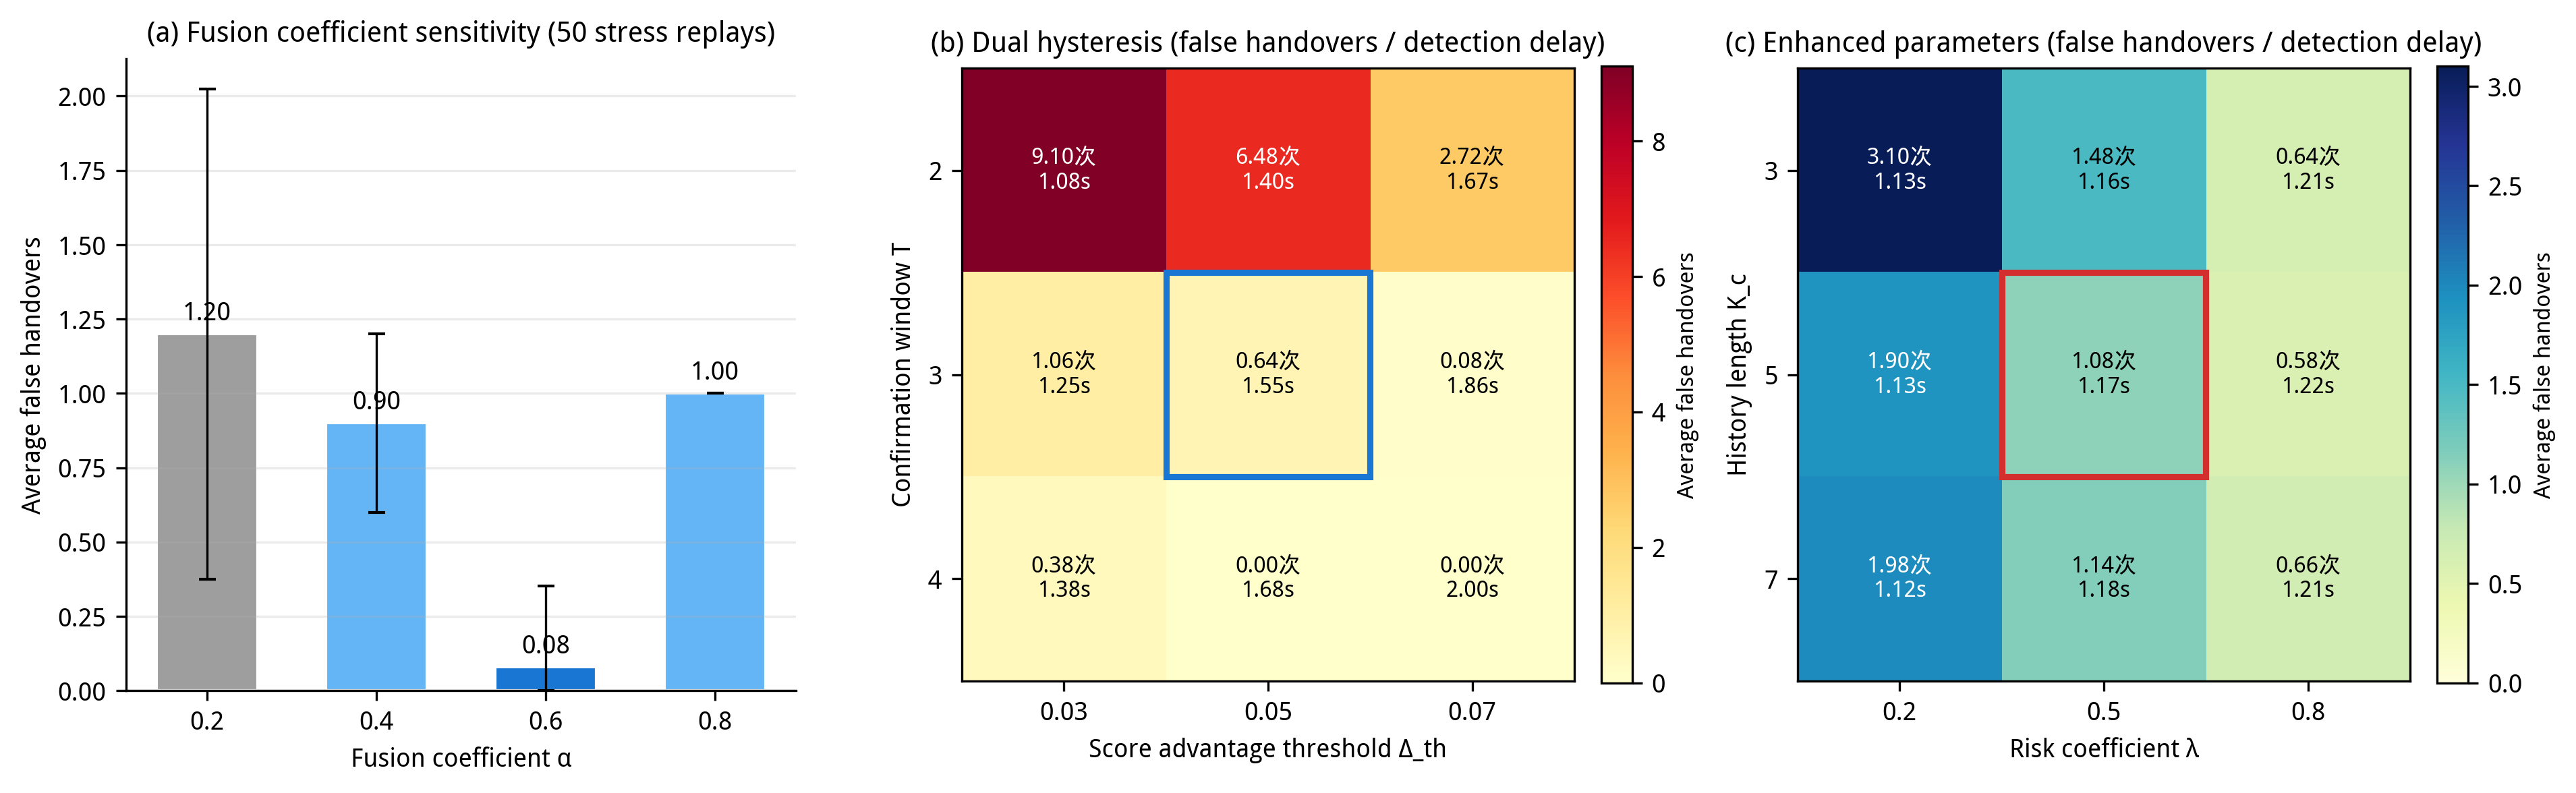
\includegraphics[width=\textwidth]{fig_parameter_sensitivity.png}
\end{figure}

在上述参数取值实验基础上，表\ref{tab:params}汇总本节采用的平台、网络场景、模型结构和训练/推理参数。后续对比算法、指标来源和结果分析均基于同一组仿真设置，以避免算法差异与实验环境差异相互混淆。

\begin{table}[H]
\centering
\caption{实验参数设置}
\small
\begin{tabular}{>{\raggedright\arraybackslash}p{3.2cm}p{8.5cm}}
\toprule
参数 & 取值 \\
\midrule
仿真平台 & ns-3.45，ns3-ai，Python/PyTorch \\
候选网络 & 5G、LTE、WiFi \\
算法范围 & LAAVHA、8种对比算法和2种消融变体 \\
运行次数 & 每种算法50组随机场景 \\
仿真时长 & $10~\mathrm{s}$ \\
决策周期 & $0.1~\mathrm{s}$ \\
每次运行决策数 & 100 \\
随机种子 & 200$\sim$249 \\
FlowMonitor模式 & feed \\
指标维度 & SINR、RSRP、时延、吞吐量、丢包率 \\
位置扰动 & $30~\mathrm{m}$ \\
高度扰动 & $10~\mathrm{m}$ \\
时间窗口$T_s$ & 10 \\
LSTM隐藏单元 & 第一层128，第二层64 \\
注意力头数（num\_heads） & 1（embed\_dim=5，采用单头注意力） \\
融合系数$\alpha$ & 0.6 \\
双重滞后参数 & $\Delta_{\mathrm{th}}=0.05$，确认窗口$T_h=3$ \\
增强机制参数 & RS-TOPSIS贴近度历史长度$K_c=5$，RS-TOPSIS风险系数$\lambda=0.5$ \\
数据集划分 & 训练/验证 = 80\%/20\% \\
优化器 & Adam \\
早停策略 & 验证集损失连续10个epoch不下降 \\
\bottomrule
\end{tabular}
\label{tab:params}
\end{table}

实验除LAAVHA外，还运行了TOPSIS-Q、Fuzzy-VHO、SAW、VIKOR、GRA、COPRAS、SPOTIS和最强信号法等8种对比算法以及LAAVHA-L、LAAVHA-A两种消融变体。这8种对比算法覆盖了模糊逻辑式（Fuzzy-VHO）、简单加权式（SAW）、补偿式（VIKOR）、距离式（TOPSIS-Q）、关联度式（GRA）、比例式（COPRAS）和参考点式（SPOTIS）七种主流决策范式，为全面评估LAAVHA的决策性能提供了多维参照。对比算法来源与设置如下：TOPSIS-Q基于TOPSIS网络选择思想及熵权改进TOPSIS方法\upcite{7--8,30}；Fuzzy-VHO参考无人机5G网络中的模糊切换机制\upcite{4}；SAW作为经典加权和MADM基线，VIKOR、GRA、COPRAS和SPOTIS选自主流MADM决策范式及其网络选择综述\upcite{11,22,30}；最强信号法为本文设置的单因素启发式基线，仅依据SINR最大原则选择候选网络。LAAVHA-L表示去除LSTM预测分支的消融变体，直接以当前状态替代预测状态，保留Attention权重与双重滞后；LAAVHA-A表示去除Attention动态权重分支的消融变体，保留LSTM预测和双重滞后，并以熵权法生成TOPSIS权重。

5G候选网络由代理链路表示，其SINR和RSRP由基于位置的传播模型计算，传输类指标来自点到点代理流的FlowMonitor统计；切换事件表示LAAVHA输出的网络编号变化，并未执行真实WiFi解除关联、LTE分离或5G新空口（NR, new radio）协议栈切换。各候选网络指标来源见表\ref{tab:metrics}。

\begin{table}[H]
\centering
\caption{候选网络指标来源}
\small
\begin{tabular}{p{1.5cm}p{3.2cm}p{2.8cm}p{3cm}p{2.5cm}}
\toprule
网络 & SINR/RSRP & 时延 & 吞吐量 & 丢包率 \\
\midrule
WiFi & 基于MobilityModel位置的传播代理值 & FlowMonitor & PacketSink区间接收字节 & FlowMonitor \\
LTE & 基于MobilityModel位置的传播代理值 & FlowMonitor & FlowMonitor & FlowMonitor \\
5G & 到假设下一代节点B（gNB, next generation NodeB）的传播代理值 & 点到点代理流FlowMonitor & 点到点代理流FlowMonitor & 点到点代理流FlowMonitor \\
\bottomrule
\end{tabular}
\label{tab:metrics}
\end{table}

表\ref{tab:metrics}用于说明第3章实验中五类网络状态指标的采集来源。SINR和RSRP主要反映物理层链路质量，实验中依据无人机与接入点或基站的相对位置及传播代理模型计算得到；时延、吞吐量和丢包率主要反映传输层服务质量，其中WiFi吞吐量由PacketSink在相邻决策周期内的接收字节数换算，LTE和5G的传输类指标由FlowMonitor统计得到。需要强调的是，该表刻画的是决策级仿真平台中的指标来源映射，而非完整协议栈实网测量流程：各候选网络在同一决策周期内提供同维度指标，随后由LAAVHA及对比算法统一归一化并输入多属性决策模块。这样设置可以保证不同算法面对完全一致的候选网络状态，避免因采集口径差异影响横向比较。

\subsection{对比算法横向比较}

为与引言提出的算法层面和遥感探测场景层面两类挑战相对应，本节结果分析也分为两个层面。第一层面验证基础算法改进的有效性：通过11种算法横向比较、代表性决策过程对比和消融实验，考察LSTM预测、注意力动态权重和双重滞后是否能够改善候选网络选择与切换稳定性。第二层面验证面向遥感探测场景的适配性：针对无人机高速跨越覆盖边界时可能出现的持续性链路劣化和信道突变，检验ALERA的ADH与RS-TOPSIS能否在保留必要切换的同时抑制误切换与乒乓切换。现有实验分别对这两个层面给出验证，不额外引入未经测量的性能指标。

为系统评估LAAVHA在不同决策范式下的性能优势，选择8种具有代表性的对比算法在同一实验条件下进行横向比较。Fuzzy-VHO基于Mamdani模糊推理系统，将SINR和RSRP模糊化后通过规则库推理输出切换决策，无需精确数学模型；SAW以固定权重对所有归一化属性进行简单加权求和，代表最基本的MADM方法；TOPSIS-Q采用熵权法确定属性权重并执行标准TOPSIS排序，不涉及时序预测；GRA通过计算各候选网络与理想参考序列的灰色关联度进行排序，对不确定性信息具有较好的处理能力；VIKOR基于折中规划思想在群体效用与个体遗憾之间寻求平衡；COPRAS对效益型和成本型指标分别评估后计算综合效用度；SPOTIS以参考点距离最小化为目标进行排序。最强信号法直接选择SINR最大的候选网络，作为单因素基线。上述11种算法对比见图\ref{fig:ho_comparison}。

\begin{figure}[H]
\centering
\caption{11种算法平均切换次数对比（mean $\pm$ std, n=50）}
\label{fig:ho_comparison}
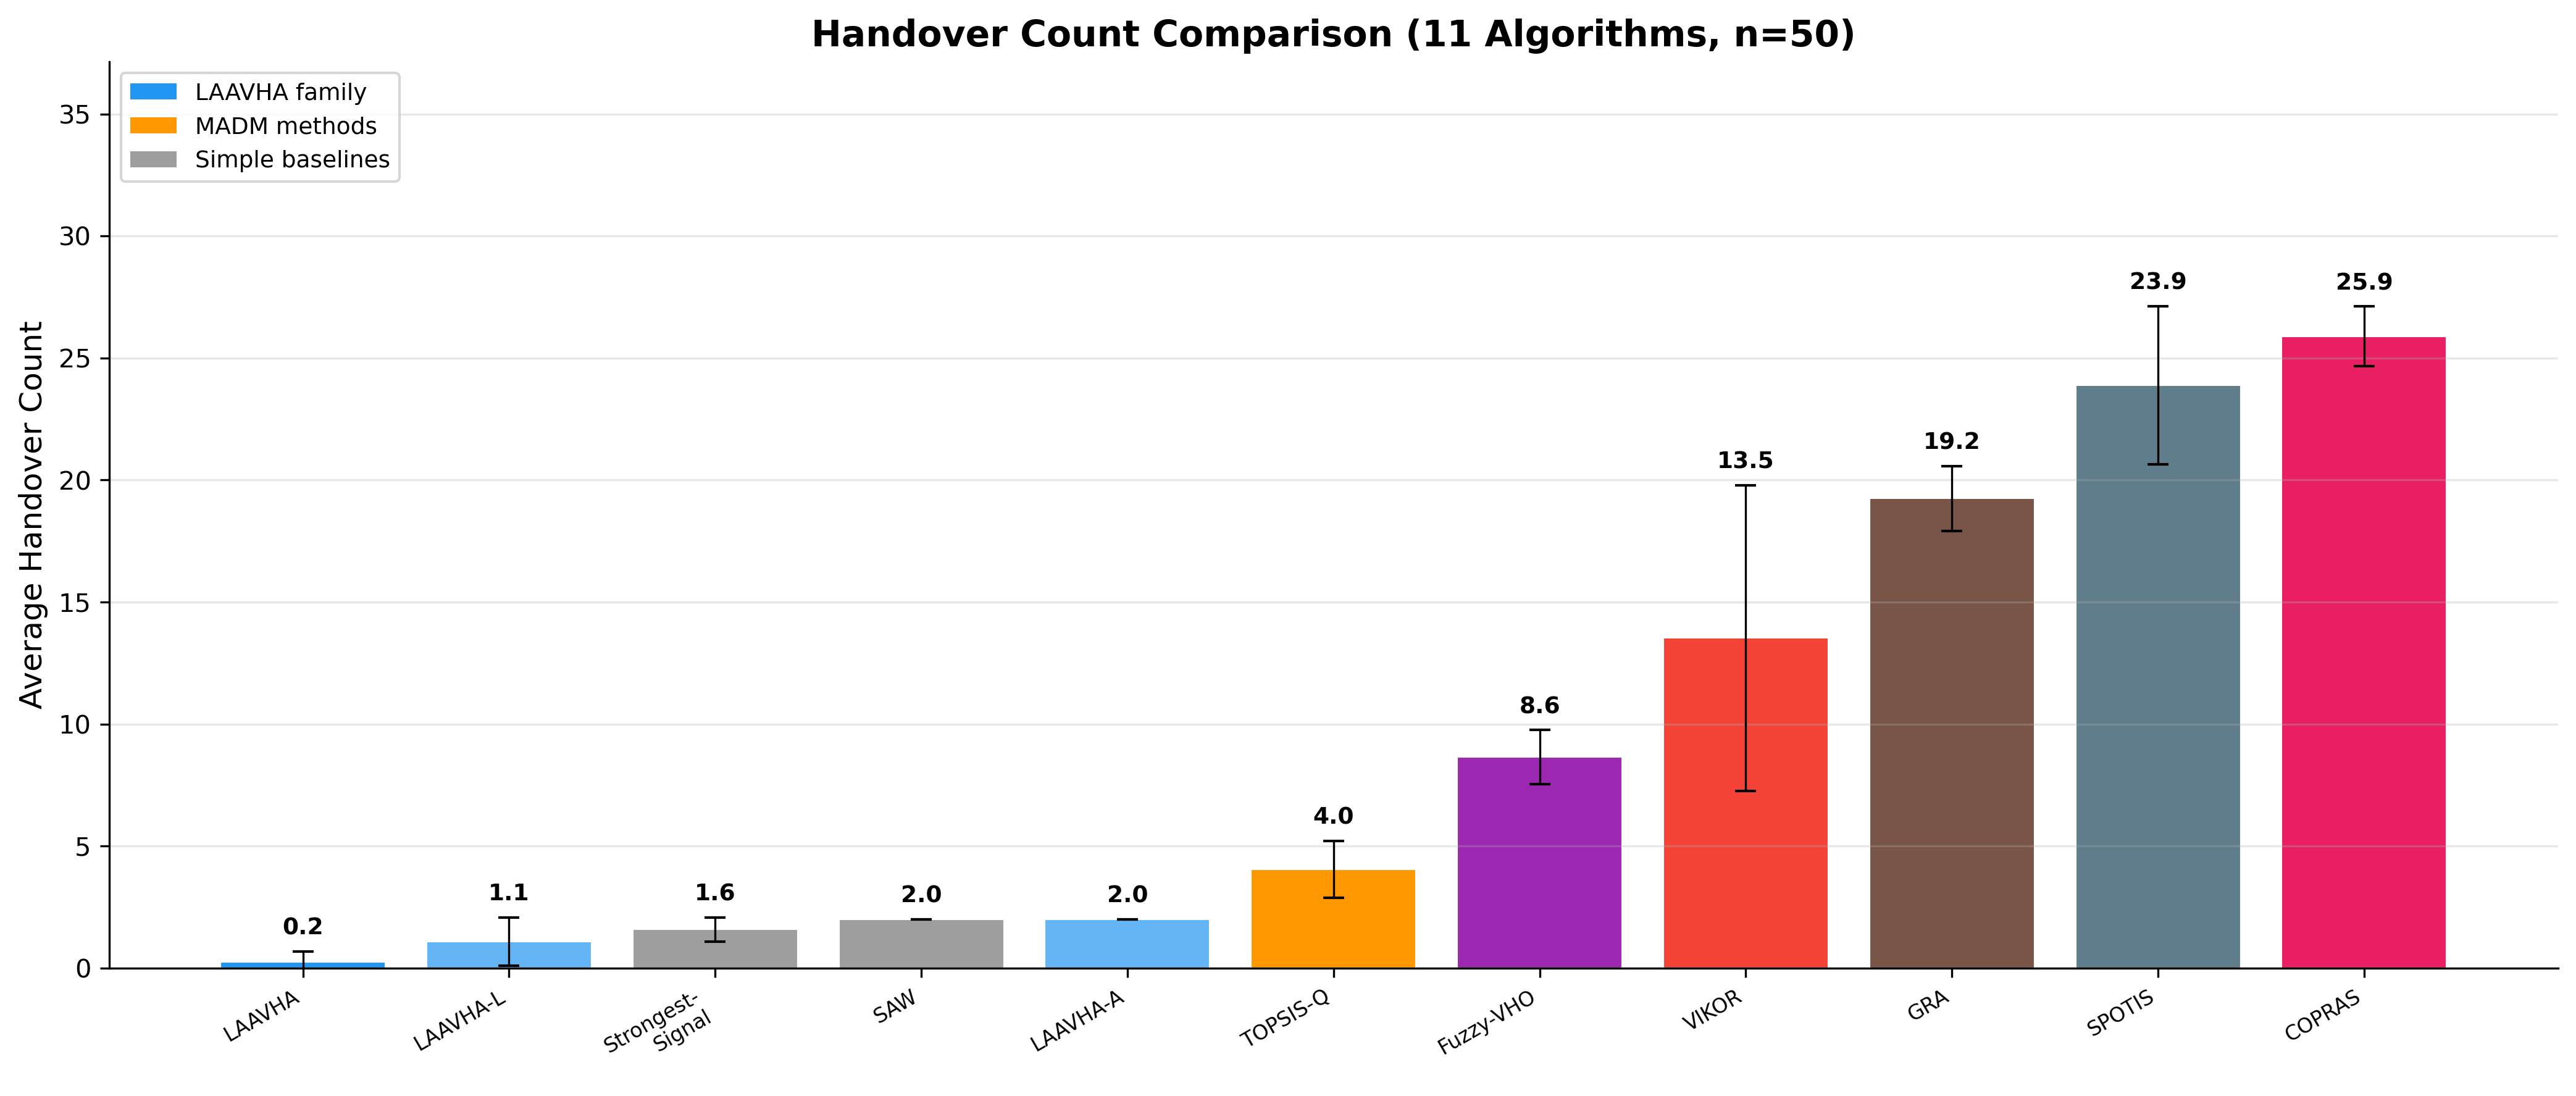
\includegraphics[width=\textwidth]{fig_handover_count_by_algorithm.png}
\end{figure}

\subsection{代表性算法决策过程对比}

图\ref{fig:scoring}以2行$\times$3列布局对比了LAAVHA、TOPSIS-Q和Fuzzy-VHO三种算法在同一随机种子（seed=200）下的决策过程。该组时序对比的目的不是单纯选择横向统计中切换次数最少的两个算法，而是选择最能解释LAAVHA改进来源的参照对象。TOPSIS-Q与LAAVHA同属TOPSIS排序框架，差异主要在于是否引入LSTM预测、Attention动态权重和双重滞后，因此二者可以形成较清晰的控制变量对比，用来观察预测状态和动态权重加入后，候选网络贴近度曲线是否更稳定、切换触发是否更克制。Fuzzy-VHO则代表另一类规则驱动方法，其决策依赖模糊隶属函数和规则库，对SINR、RSRP等局部波动更敏感；将其与LAAVHA并列，可以从不同决策范式角度展示动态多属性融合方法相对于规则式切换方法的鲁棒性。相较之下，最强信号法和SAW虽然在平均切换次数上可能较低，但前者只依据单一SINR，后者采用固定加权求和，缺少可与LAAVHA内部评分机制对应的时序解释维度，因此更适合作为总体统计基线，而不适合作为图\ref{fig:scoring}中的机制分析对象。上排三幅子图的纵轴为贴近度（Closeness Score），展示5G、LTE和WiFi三个候选网络在TOPSIS排序中的综合得分变化；贴近度越接近1，表示该网络对遥感任务的综合保障能力越强。下排三幅子图的纵轴为SINR（dB），展示同一仿真中三个网络的物理层信号质量变化。红色竖虚线标记切换发生时刻。可以观察到，LAAVHA的5G贴近度在全过程中保持稳定高水平（0.99$\sim$1.00），LTE和WiFi评分均远低于5G，结合双重滞后机制（$\Delta_{\mathrm{th}}=0.05, T_h=3$）全程未触发任何切换。尽管下排SINR子图显示5G信号并非始终最高，但注意力机制生成的动态权重综合了时延、吞吐量和丢包率等多维指标后仍然选择5G，体现了多属性融合决策的优势。相比之下，TOPSIS-Q在5G与WiFi贴近度接近时发生了数次切换，Fuzzy-VHO因模糊规则对SINR波动敏感而产生多次切换；这一结果直观展示了时序预测和动态权重对决策稳定性的关键贡献。

\begin{figure}[H]
\centering
\caption{LAAVHA/TOPSIS-Q/Fuzzy-VHO候选网络评分与SINR时序对比（seed=200，竖线=切换时刻）}
\label{fig:scoring}
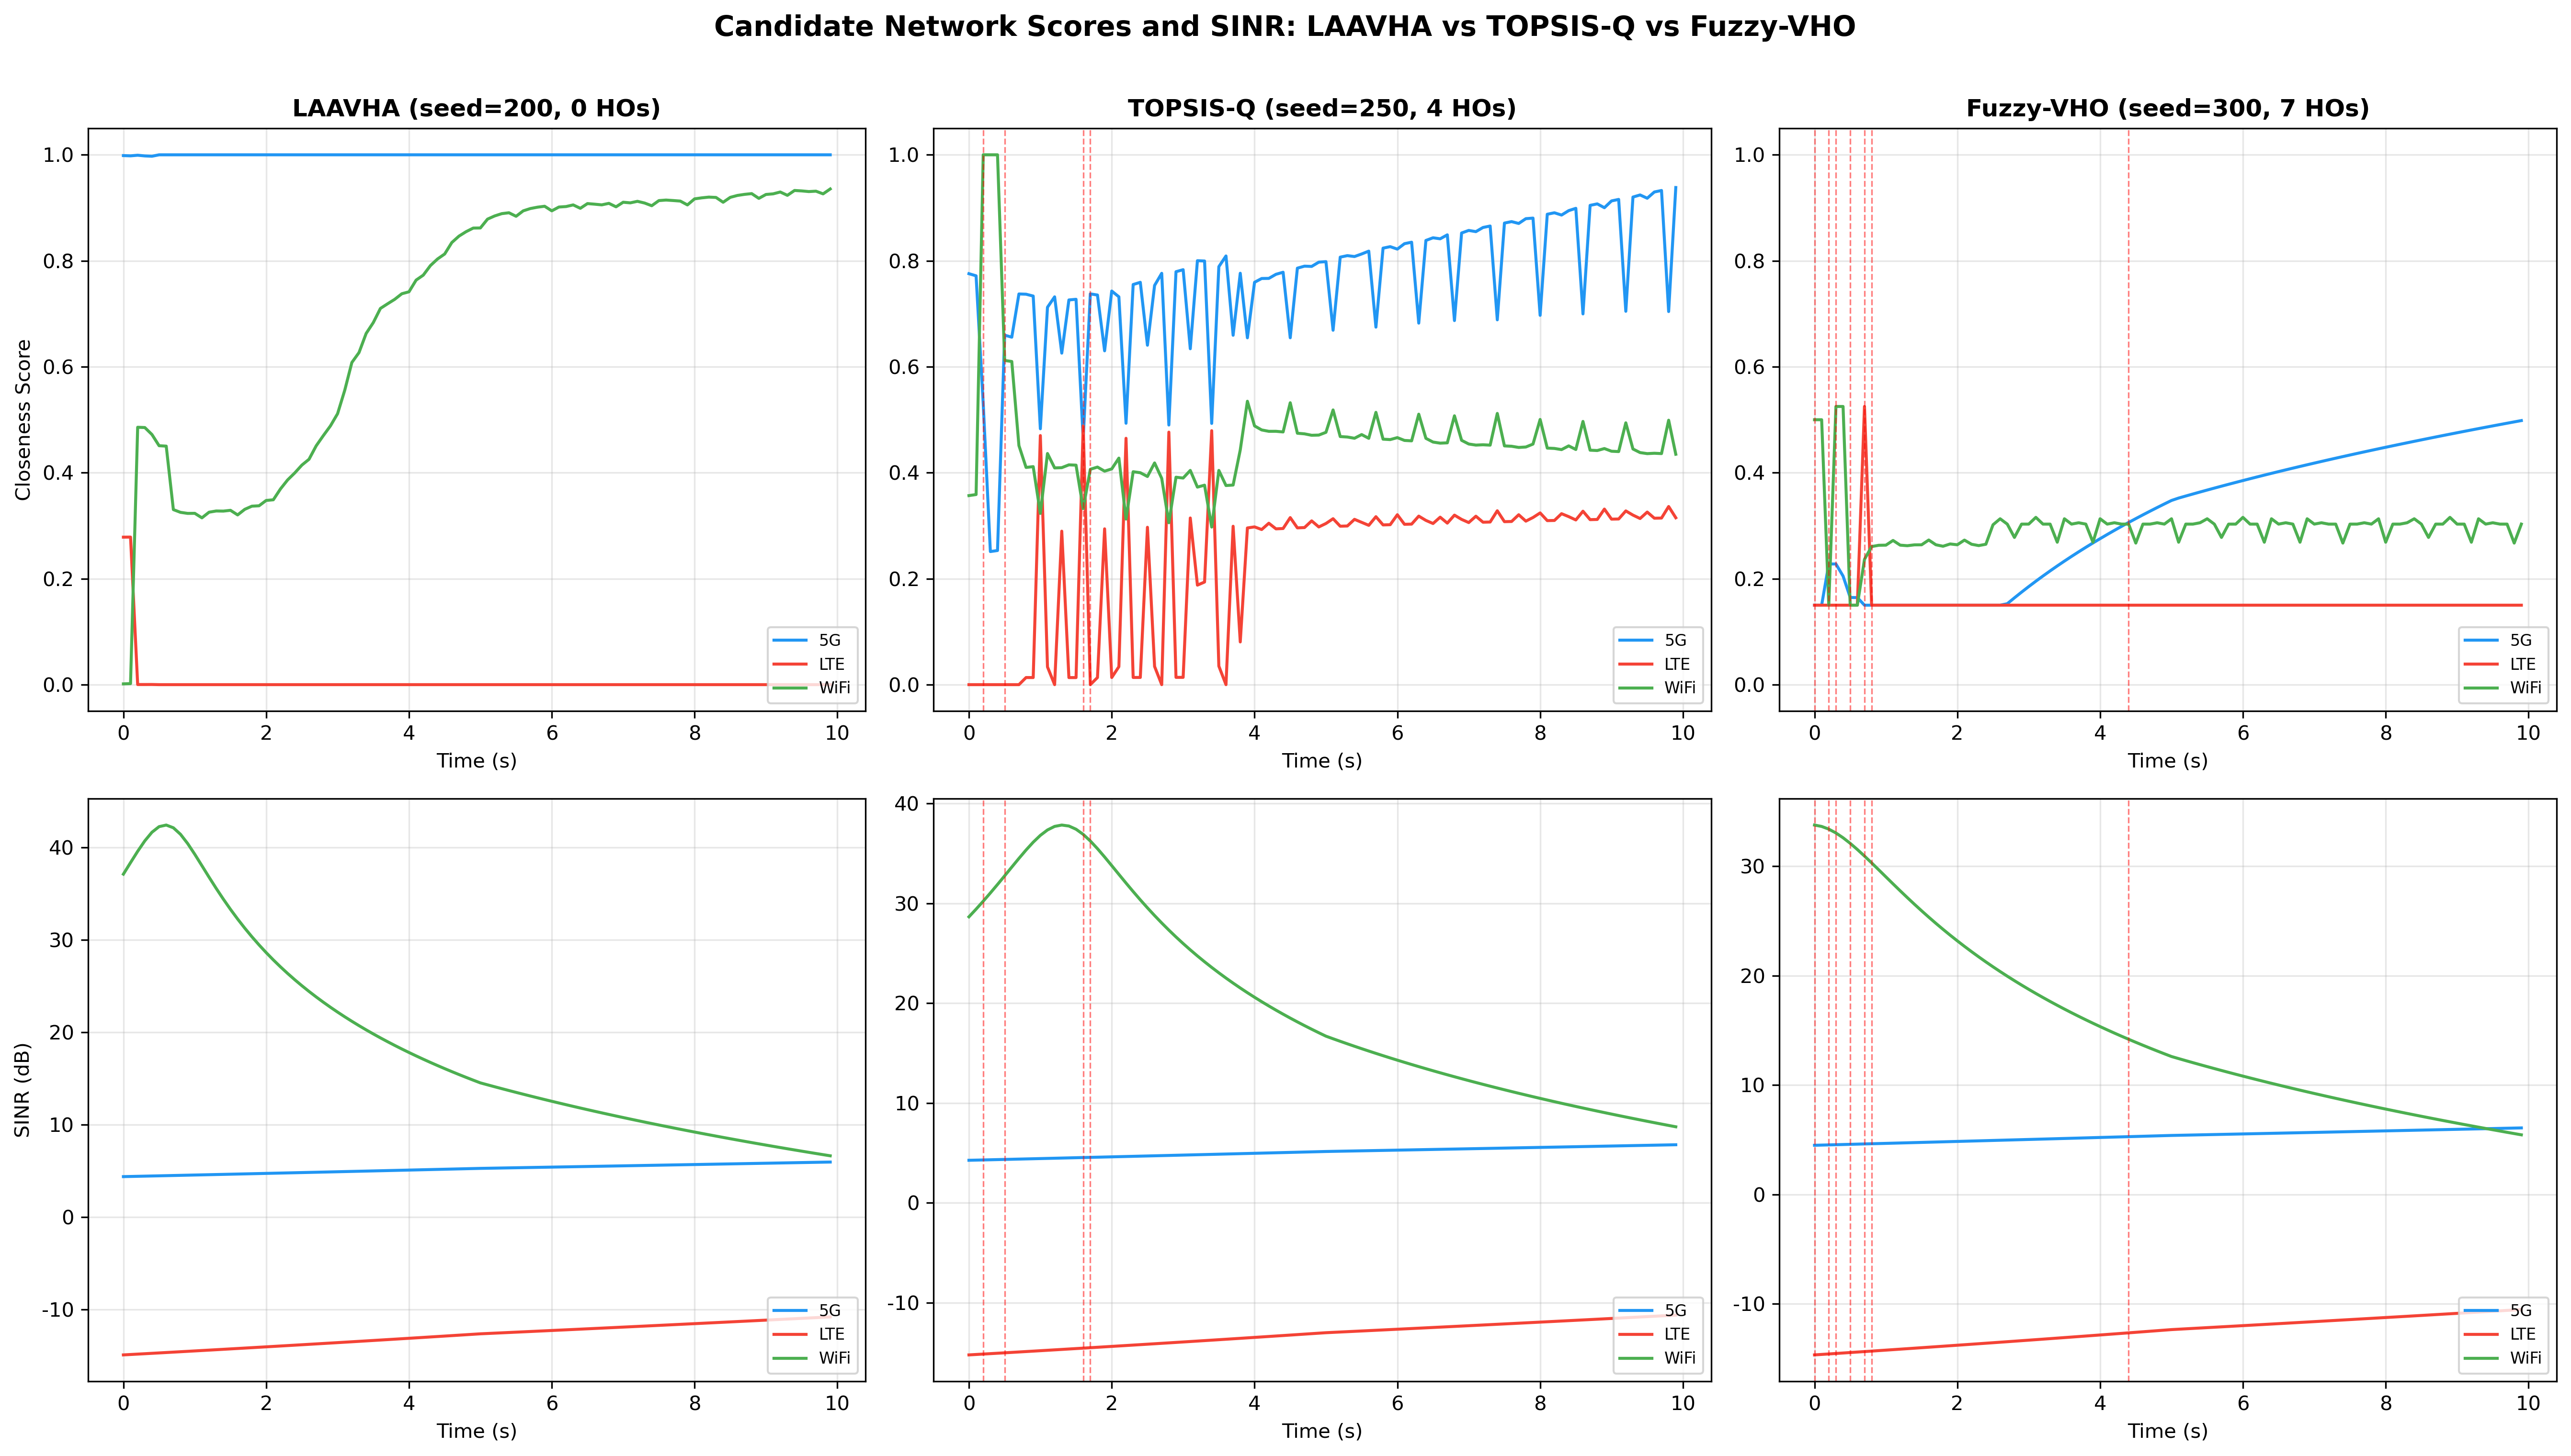
\includegraphics[width=\textwidth]{fig_scoring_timeline_comparison.png}
\end{figure}

\subsection{消融实验验证}

为量化LSTM预测模块和注意力动态权重模块对LAAVHA决策质量的贡献，设计消融实验。LAAVHA-L为移除LSTM预测分支的版本，直接令预测状态等于当前状态，仅保留Attention权重生成、改进TOPSIS和双重滞后逻辑，用于检验短期状态预测的作用；LAAVHA-A为移除Attention动态权重分支的版本，保留LSTM预测、改进TOPSIS和双重滞后逻辑，但采用熵权法替代Attention输出权重，用于检验动态权重学习的作用。两组消融变体与完整LAAVHA在相同的50组随机种子（200$\sim$249）和仿真参数下运行。图\ref{fig:ablation}以散点叠加柱状图的形式展示了三种方案的切换次数对比，其中每个散点代表一次独立运行的结果，柱高为均值，误差线为$\pm1$标准差。完整LAAVHA平均切换仅0.24次（std=0.43），50次运行中38次保持零切换、12次出现1次切换，体现了LSTM预测与注意力动态权重协同工作的决策稳定性；LAAVHA-L（去LSTM）平均切换1.08次（std=1.01），失去时序预测后算法退化为被动反应式决策，切换次数显著升高且方差增大；LAAVHA-A（去Attention）平均切换2.00次（std=0.00），全部50次运行均产生2次切换，说明仅依靠熵权难以根据飞行阶段自适应调整评价标准，在WiFi覆盖边缘必然触发乒乓切换。

\begin{figure}[H]
\centering
\caption{LAAVHA消融实验切换次数对比（mean $\pm$ std, n=50）}
\label{fig:ablation}
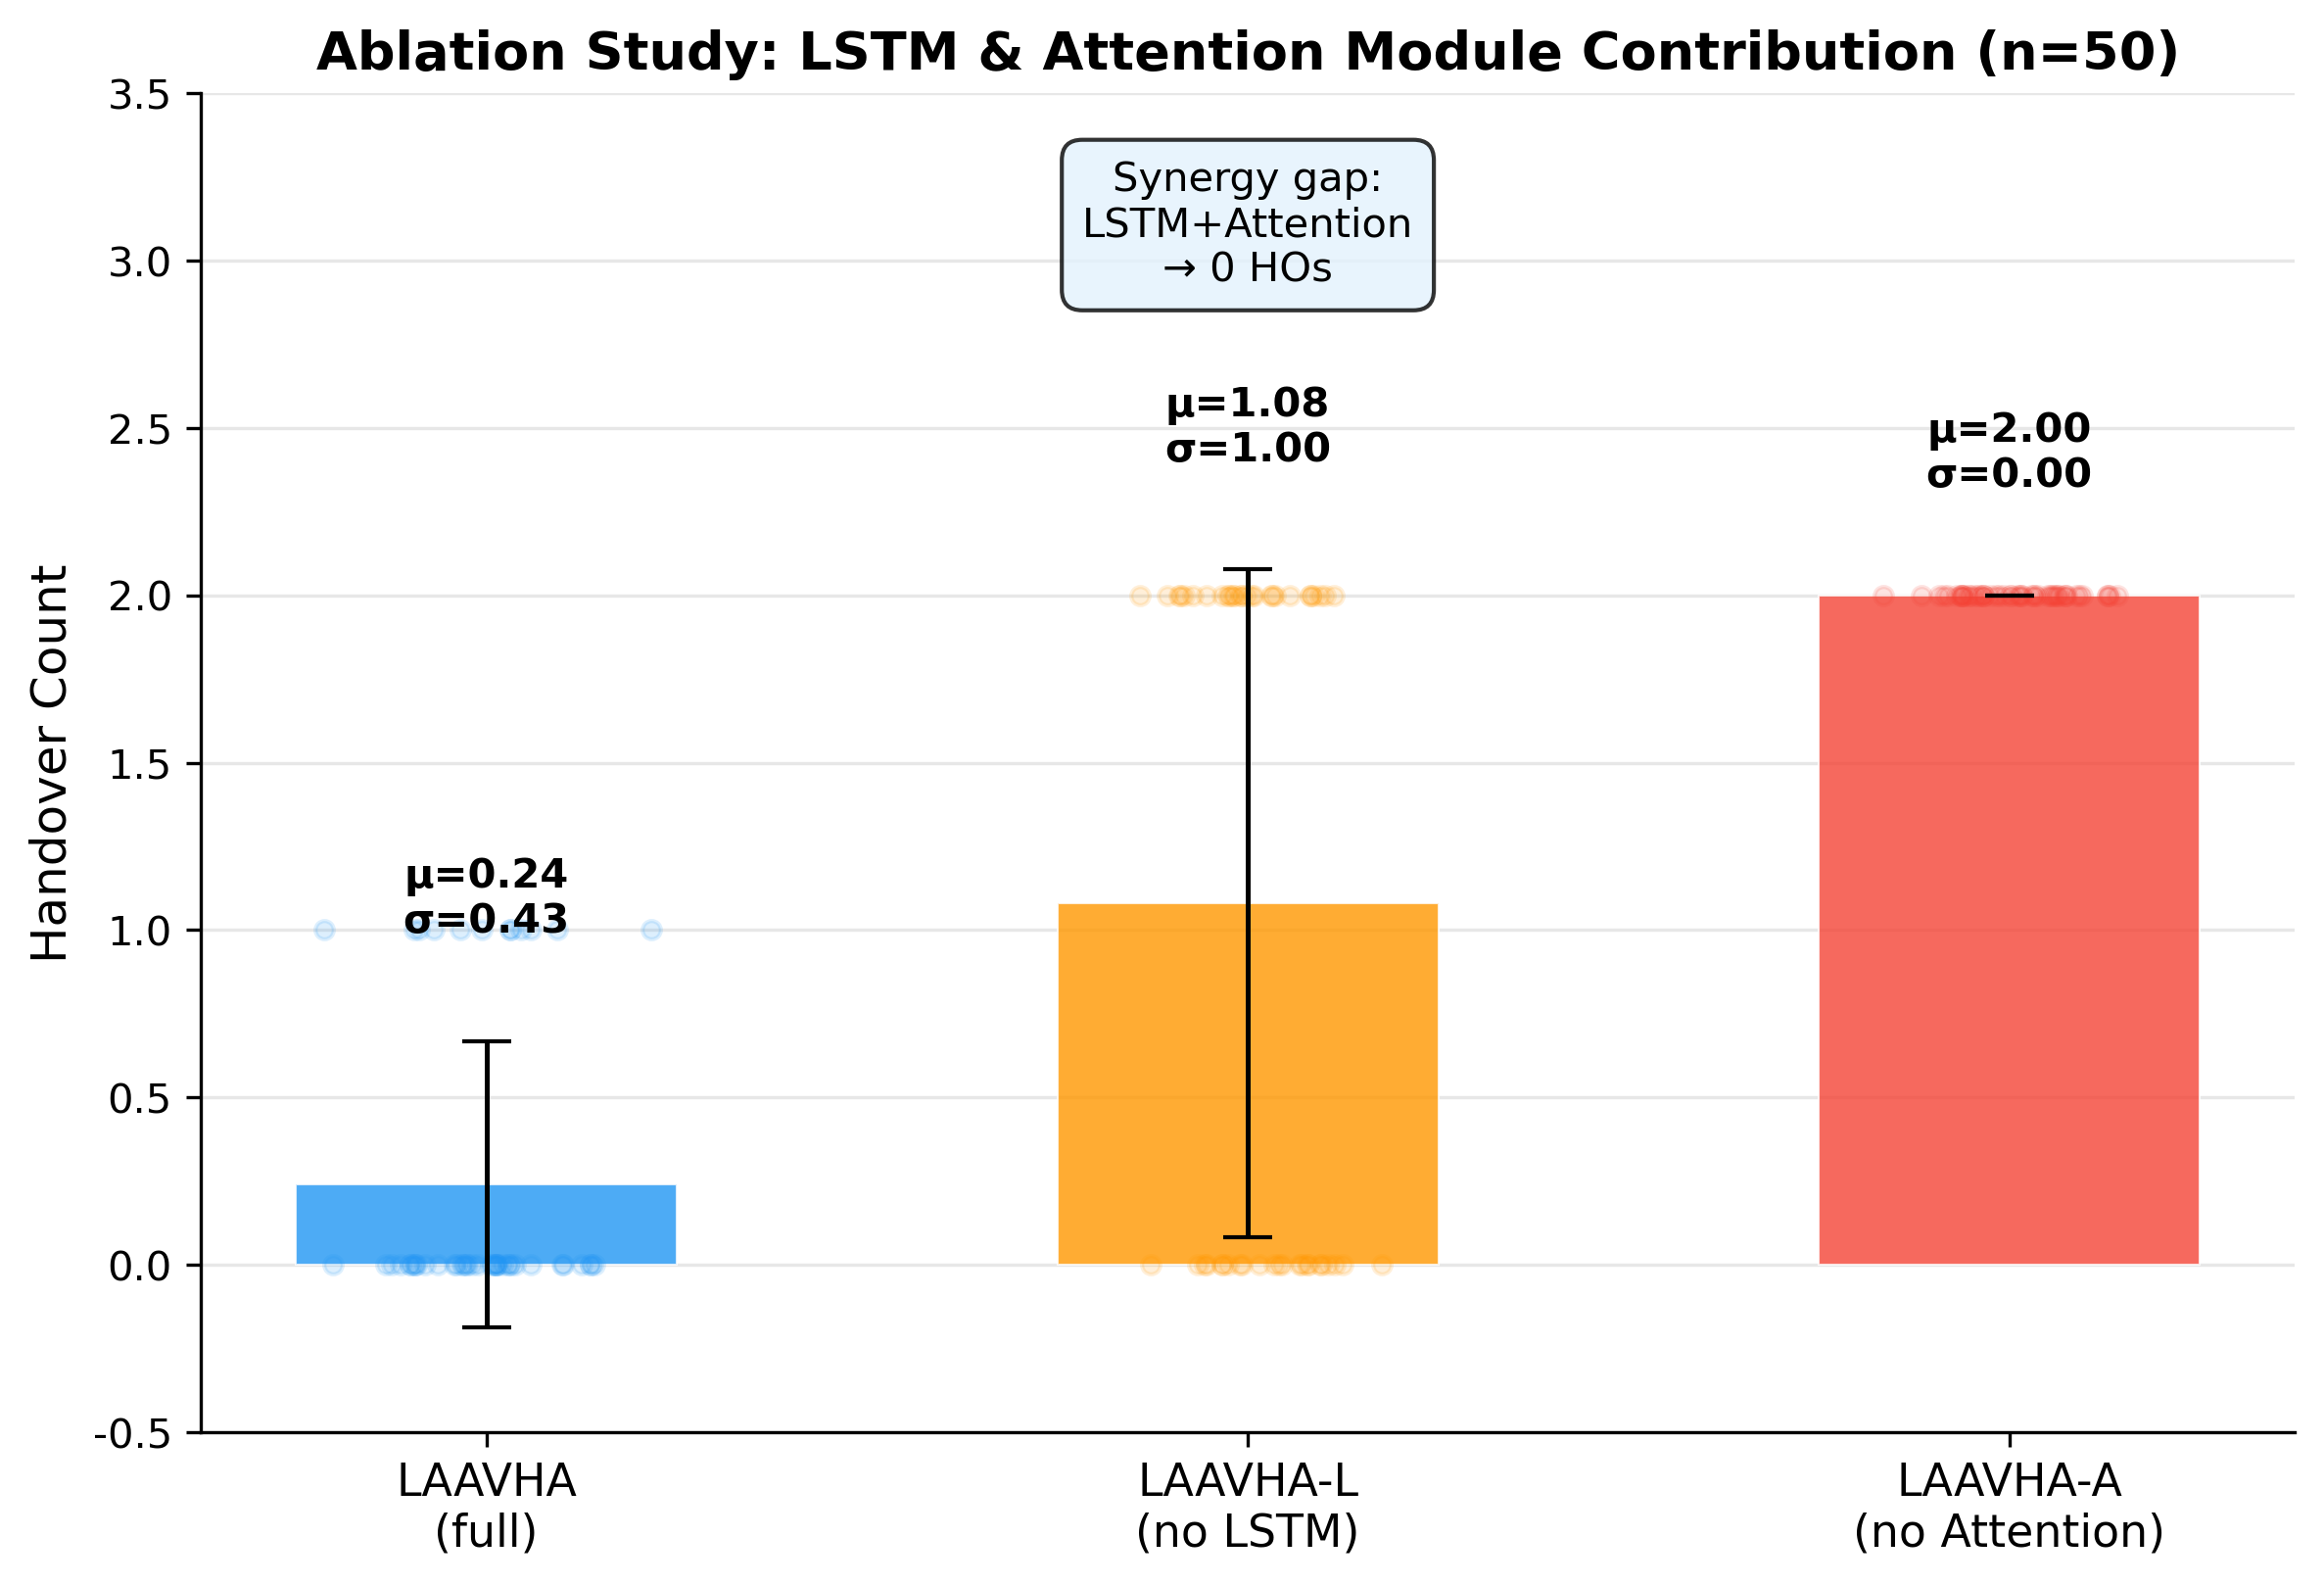
\includegraphics[width=0.68\textwidth]{fig_laavha_handover_count.png}
\end{figure}

上述消融结果表明，LSTM预测模块和注意力动态权重模块对LAAVHA决策质量的贡献具有显著的协同效应：单独保留任一模块均无法维持低切换水平。Attention模块的缺失影响最为严重（平均切换从0.24次增至2.00次，增幅达8倍，且50次运行无一例外），说明在遥感巡航场景下，基于飞行状态和候选网络状态生成的动态权重比静态统计权重更能区分不同飞行阶段的网络需求；LSTM模块的缺失导致切换次数上升至1.08次且方差增大（std=1.01），说明时序预测能力对维持决策稳定性同样关键。两个模块的消融结果从正反两面共同验证了LAAVHA架构设计的合理性。

\subsection{遥感探测场景适配性与增强机制验证}

为验证ALERA对遥感探测场景中快速跨越覆盖边界和信道突变的适配能力，构造网络A（类比5G）与网络B（类比WiFi）贴近度在0.50附近拉锯的竞争场景，初始状态设为接入网络A。该场景抽象了无人机持续回传遥感图像时所面临的两类典型情况：覆盖条件持续恶化时必须及时迁移，以及短时遮挡或多径扰动引起瞬时波动时应避免无效切换。图\ref{fig:enhanced}给出了同一时间轴下的四个子图，横坐标统一对应最下方的时间轴，因而图\ref{fig:enhanced}-a到图\ref{fig:enhanced}-d中$t=5\sim8~\mathrm{s}$和$t=12\sim15~\mathrm{s}$表示同一段仿真时间。浅蓝色区域Zone 1表示持续性链路劣化区间，即网络A的综合服务质量在一段时间内持续下降、网络B持续改善，因此从A切换到B属于必要且正确的切换；浅红色区域Zone 2表示瞬时波动区间：网络B被注入正弦振荡和高斯噪声，虽然会出现短时峰值，但其均值并未形成稳定优势，因此不应触发切换。

图\ref{fig:enhanced}-a展示两个网络的原始贴近度（Closeness）曲线，纵坐标表示未进行风险惩罚前的候选网络综合评分，数值越大表示该网络越接近理想候选网络。可以看到，Zone 1中网络B的优势是连续形成的，而Zone 2中网络B只是高频振荡造成的瞬时抬升。

图\ref{fig:enhanced}-b展示固定低阈值方案（$\Delta_{\mathrm{th}}=0.03$）的切换结果，纵坐标仍为原始贴近度，红色虚线表示实际执行的切换时刻，图中已标明切换方向。该方案在$t=6.6~\mathrm{s}$执行A$\rightarrow$B、在$t=11.9~\mathrm{s}$执行B$\rightarrow$A，这两次分别对应Zone 1中的持续性链路劣化和劣化结束后的恢复，属于正确切换；但在Zone 2内又于$t=14.8~\mathrm{s}$执行A$\rightarrow$B、$t=15.1~\mathrm{s}$执行B$\rightarrow$A，这两次仅由网络B的瞬时峰值触发，未对应链路质量的持续改善，因而属于误切换和随后的乒乓切换。

图\ref{fig:enhanced}-c展示ALERA增强机制下的LCB调整后评分，纵坐标为$C_i^{\mathrm{robust}}=C_i-\lambda\sigma_i^C$，即在原始贴近度基础上扣除了历史波动风险罚分后的排序分数；绿色虚线表示增强机制实际执行的切换时刻。可以看到，ALERA仍然保留了Zone 1中的A$\rightarrow$B正确切换和劣化结束后的B$\rightarrow$A恢复切换，说明增强机制并未因为提高鲁棒性而阻塞必要切换；同时，Zone 2内网络B的高频振荡被风险罚分压低，未触发任何切换。

图\ref{fig:enhanced}-d展示自适应阈值$\Delta_{\mathrm{th}}$随时间变化，纵坐标表示当前切换判决所需的最小贴近度优势。Zone 2波动期间，阈值由基线0.03自动抬升至约0.09，显著高于固定低阈值方案；波动消退后阈值逐步回落，说明ADH只在波动场景下提高切换门槛。

从网络切换正确性看，增强机制的优势体现在两个方面：一是面对持续性链路劣化时仍能完成必要切换，保证无人机从劣化网络A迁移到更优网络B，避免因过度保守导致服务质量下降；二是面对瞬时波动时能够拒绝短时峰值诱导的误切换，避免A$\rightarrow$B$\rightarrow$A的乒乓过程。RS-TOPSIS负责在``切向谁''的问题上压低高波动候选网络的排序优势，ADH负责在``何时切换''的问题上提高波动阶段的触发门槛，两者共同使算法既保持正确切换能力，又减少错误切换和由此带来的链路重建开销。

\begin{figure}[H]
\centering
\caption{自适应滞后机制验证：固定低阈值（$\Delta_{\mathrm{th}}=0.03$）与ALERA在持续性链路劣化和瞬时波动竞争场景下的对比}
\label{fig:enhanced}
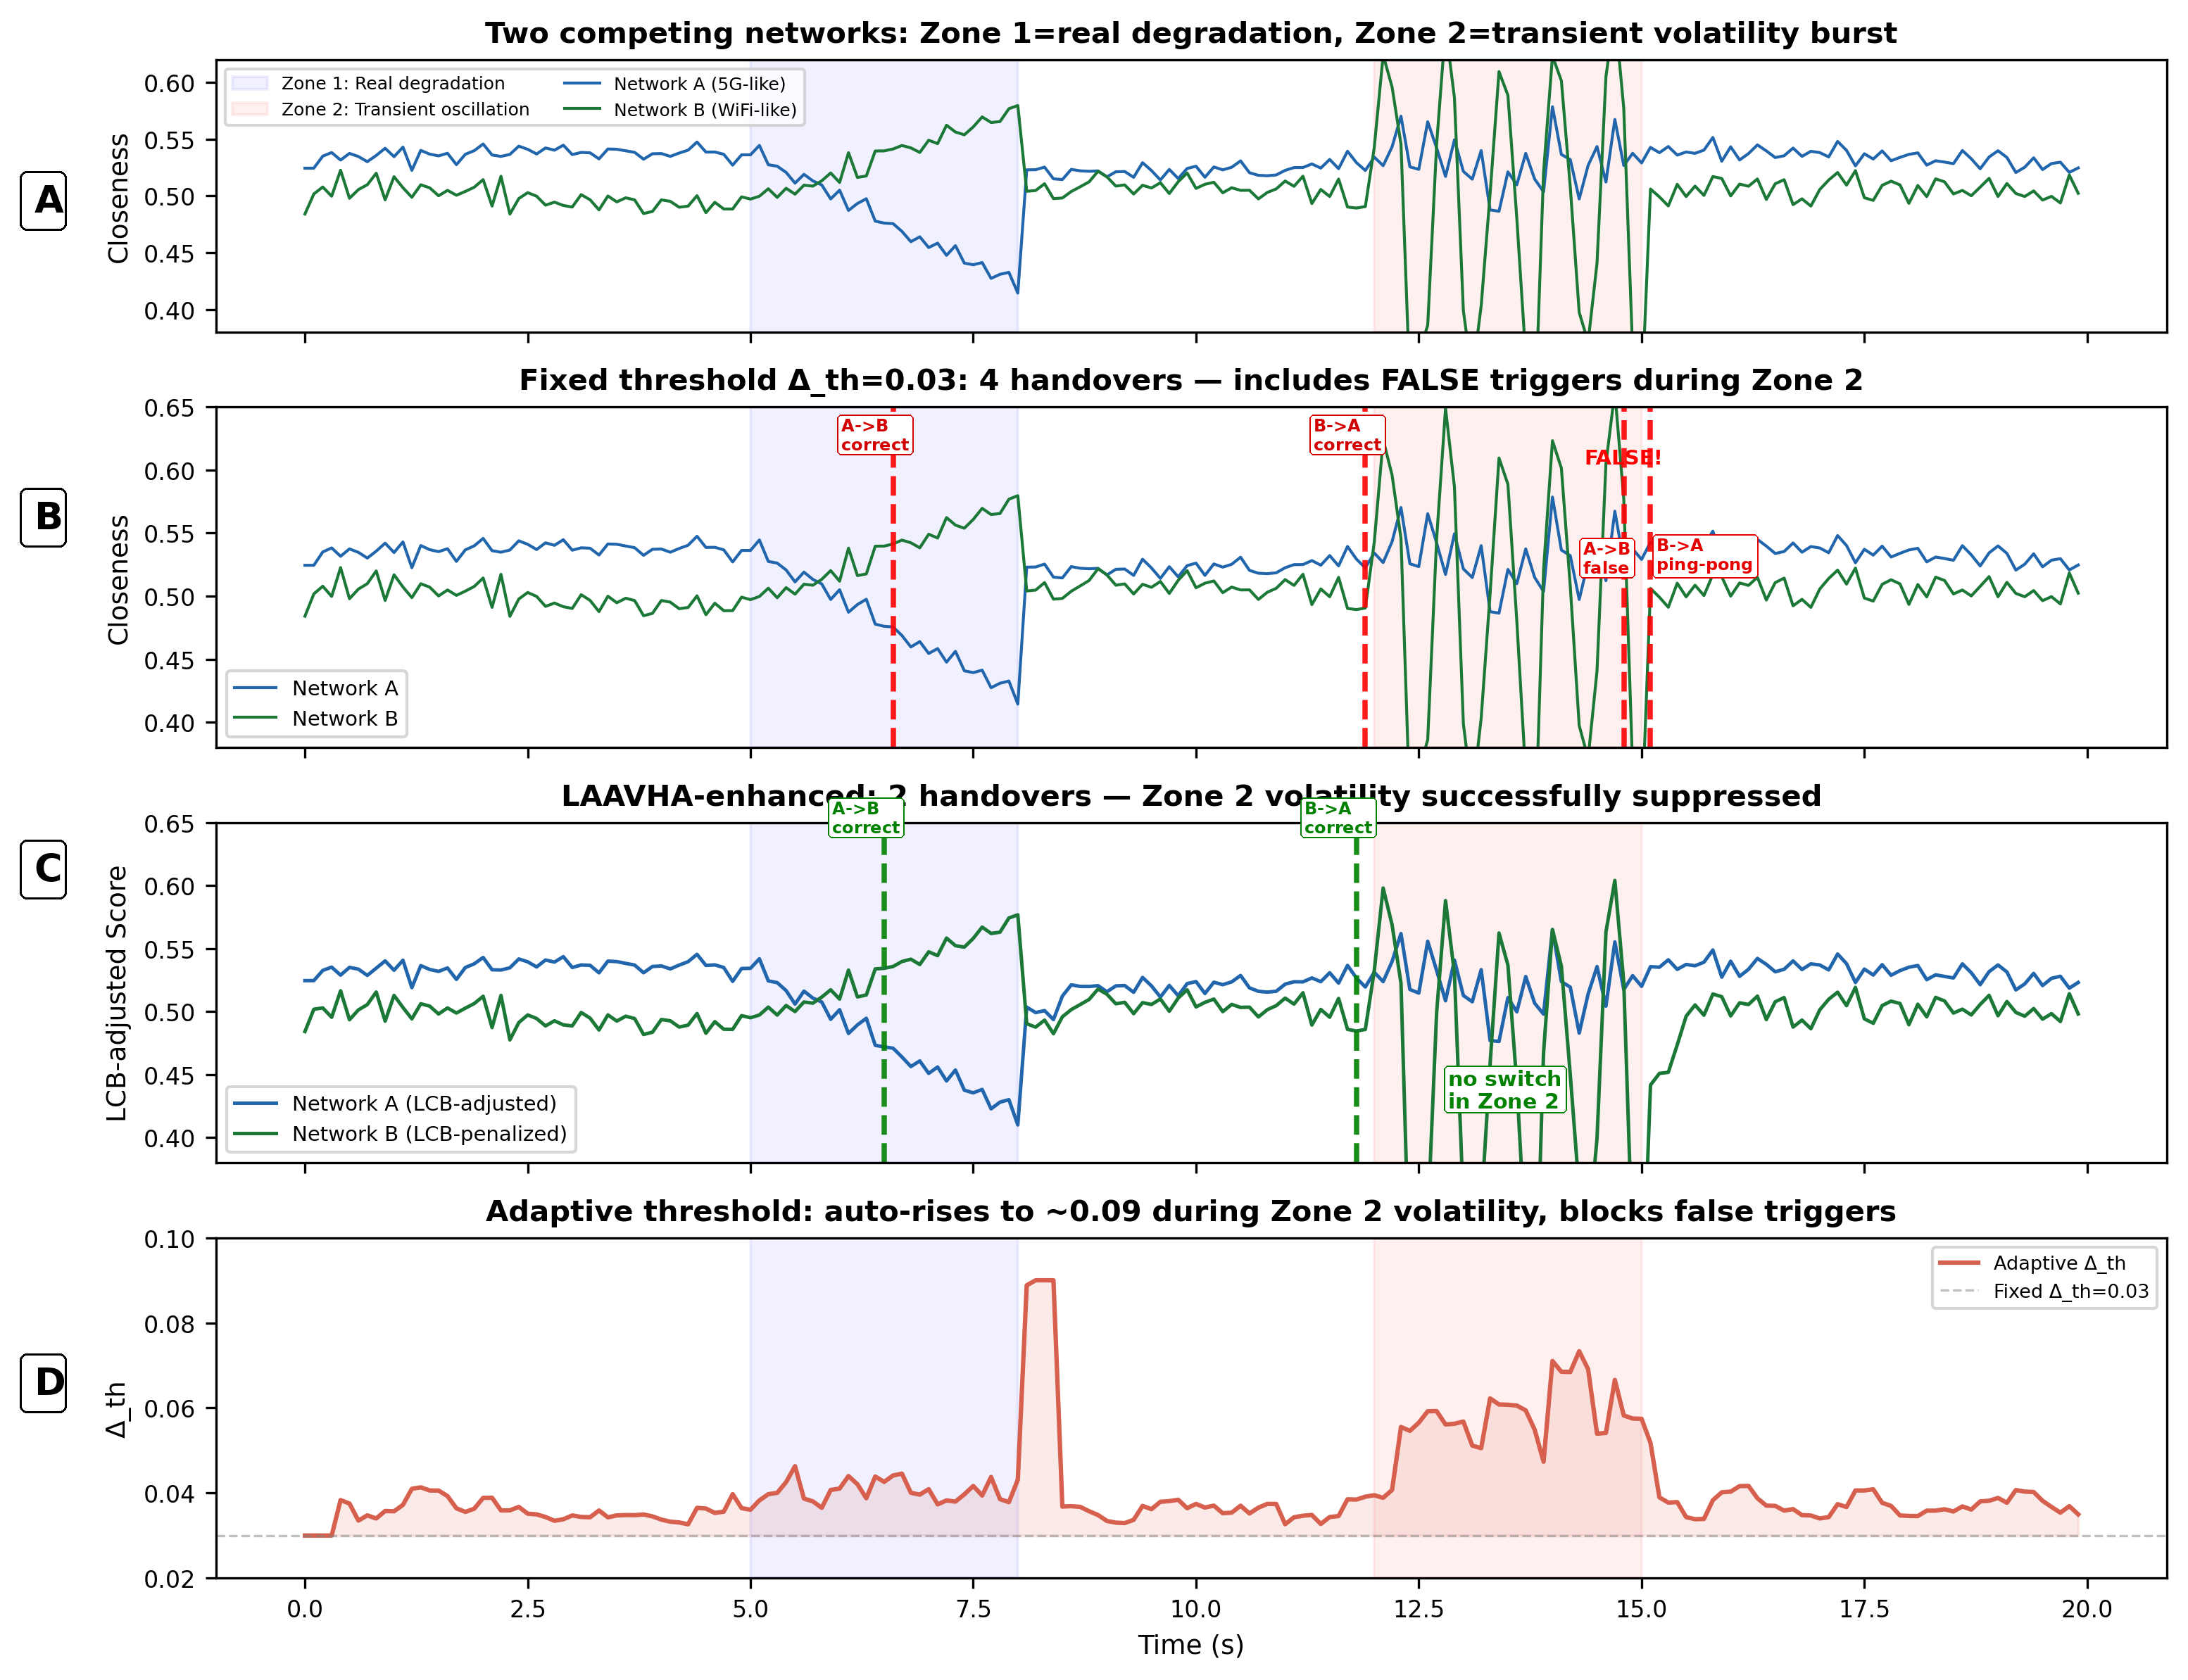
\includegraphics[width=0.86\textwidth]{fig_adaptive_hysteresis_proof.png}
\end{figure}

\section{结束语}

面向无人机遥感监测中广域飞行、异构覆盖和链路状态快速变化带来的垂直切换问题，本文提出了基于LSTM-Attention的LAAVHA自适应垂直切换方法，并在其决策层进一步构建增强型风险感知垂直切换算法ALERA。LAAVHA以5G、LTE和WiFi候选网络的SINR、RSRP、时延、吞吐量和丢包率作为统一状态输入，将历史状态序列$X_k$输入堆叠LSTM得到短期预测状态$S_{\mathrm{pred}}$，将当前状态矩阵$S_{\mathrm{cur}}$和移动状态输入注意力模块得到动态权重$w$，再通过融合当前与预测状态的改进TOPSIS计算候选网络贴近度$C_i$，最后结合双重滞后机制输出切换决策。ALERA在不改变LSTM-Attention模型结构和不重新训练参数的前提下，进一步引入自适应滞后（ADH）和风险敏感TOPSIS（RS-TOPSIS）：前者根据当前服务网络近期SINR波动度和飞行速度动态调整切换阈值$\Delta_{\mathrm{th}}$与确认窗口$T_h$，后者基于贴近度历史波动对候选网络评分施加置信下界风险惩罚。由此，全文形成了状态采集、时序预测、动态加权、融合排序、滞后裁定与风险增强的连续决策链路，使每个模块的输出都成为后续模块的输入，同时兼顾了深度学习的前瞻建模能力和TOPSIS决策过程的可解释性。

基于由ns-3.45与ns3-ai搭建的决策级协同仿真平台，本文在50组随机种子、每组100个决策周期的设置下，对LAAVHA、8种对比算法和2种消融变体进行了横向比较。仿真结果从两个层面对前文的设计形成验证：在算法层面，时序预测、动态权重和双重滞后的协同作用能够提高切换稳定性。在遥感探测场景适配层面，ALERA能在覆盖条件持续劣化时完成必要切换、在发生信道瞬时波动时抑制误切换和乒乓切换，表明ADH与RS-TOPSIS分别从``何时切换''和``切向谁''两个环节增强了无人机遥感数据持续回传过程中的抗扰能力。需要指出的是，本文实验仍属于决策级验证，5G链路和切换事件采用代理建模方式表示；后续工作将进一步结合更完整的协议栈切换过程和真实飞行轨迹数据，验证LAAVHA/ALERA在实网异构接入场景中的时延开销、链路重建代价和遥感数据传输完整性。

\section*{参考文献}
{\renewcommand{\refname}{}
\vspace{-2.5em}
\begin{thebibliography}{30}
\bibitem{ref1} YANG K, WANG Y, GAO X, et al. Communications in space-air-ground integrated networks: an overview[J]. Space: Science \& Technology, 2025, 5: 0199.
\bibitem{ref2} MOZAFFARI M, SAAD W, BENNIS M, et al. A tutorial on UAVs for wireless networks: applications, challenges, and open problems[J]. IEEE Communications Surveys \& Tutorials, 2019, 21(3): 2334--2360.
\bibitem{ref3} RIBEIRO L M B, MÜLLER I, BECKER L B. Communication interface manager for improving performance of heterogeneous UAV networks[J]. Sensors, 2021, 21(13): 4255.
\bibitem{ref4} AYASS T, COQUEIRO T, CARVALHO T, et al. Unmanned aerial vehicle with handover management fuzzy system for 5G networks: challenges and perspectives[J]. Intelligence \& Robotics, 2022, 2(1): 20--36.
\bibitem{ref5} WANG Z, LV Z, XU X, et al. Vertical switching algorithm for unmanned aerial vehicle in power grid heterogeneous communication networks[J]. Electronics, 2024, 13(13): 2612.
\bibitem{ref6} ALAM S, SULISTYO S, MUSTIKA I W, et al. Handover decision for V2V communication in VANET based on moving average slope of RSS[J]. Journal of Communications, 2021, 16(7): 284--293.
\bibitem{ref7} GOUTAM S, UNNIKRISHNAN S, KARANDIKAR A. Algorithm for handover decision based on TOPSIS[C]//2020 International Conference on UK-China Emerging Technologies. Piscataway: IEEE Press, 2020: 1--4.
\bibitem{ref8} XIAO K Y, LI C G. Vertical handoff decision algorithm for heterogeneous wireless networks based on entropy and improved TOPSIS[C]//2018 IEEE 18th International Conference on Communication Technology. Piscataway: IEEE Press, 2018: 706--710.
\bibitem{ref9} AHMED I I O, IPAYE A A, MITROPOULOS D N G, et al. Vertical handover E-TOPSIS algorithm mathematical model using AHP and standard deviation weighing method[C]//2019 International Conference on Computer, Control, Electrical, and Electronics Engineering. Piscataway: IEEE Press, 2019: 1--5.
\bibitem{ref10} SATAPATHY P, MAHAPATRO J. An efficient multicriteria-based vertical handover decision-making algorithm for heterogeneous networks[J]. Transactions on Emerging Telecommunications Technologies, 2022, 33(4): e4409.
\bibitem{ref11} DANTAS SILVA F S, LIMA M P S, CORUJO D, et al. A comprehensive step-wise survey of multiple attribute decision-making mobility approaches[J]. IEEE Access, 2024, 12: 108616--108656.
\bibitem{ref12} TAN K, BREMNER D, LE KERNEC J, et al. Intelligent handover algorithm for vehicle-to-network communications with double-deep Q-learning[J]. IEEE Transactions on Vehicular Technology, 2022, 71(7): 7848--7862.
\bibitem{ref13} JANG Y, RAZA S M, KIM M, et al. Proactive handover decision for UAVs with deep reinforcement learning[J]. Sensors, 2022, 22(3): 1200.
\bibitem{ref14} ZAID M, KADIR M K A, SHAYEA I, et al. Machine learning-based approaches for handover decision of cellular-connected drones in future networks: a comprehensive review[J]. Engineering Science and Technology, an International Journal, 2024, 55: 101732.
\bibitem{ref15} HOCHREITER S, SCHMIDHUBER J. Long short-term memory[J]. Neural Computation, 1997, 9(8): 1735--1780.
\bibitem{ref16} KAUR G, GOYAL R K, MEHTA R. An efficient handover mechanism for 5G networks using hybridization of LSTM and SVM[J]. Multimedia Tools and Applications, 2022, 81(26): 37057--37085.
\bibitem{ref17} MOLLEL M S, ABUBAKAR A I, OZTURK M, et al. A survey of machine learning applications to handover management in 5G and beyond[J]. IEEE Access, 2021, 9: 45770--45802.
\bibitem{ref18} SOYDANER D. Attention mechanism in neural networks: where it comes and where it goes[J]. Neural Computing and Applications, 2022, 34(16): 13371--13385.
\bibitem{ref19} MANZOOR S, MANZOOR M, MANZOOR H, et al. Which simulator to choose for next generation wireless network simulations? ns-3 or OMNeT++[J]. Engineering Proceedings, 2023, 46(1): 36.
\bibitem{ref20} YIN H, LIU P, LIU K, et al. ns3-ai: fostering artificial intelligence algorithms for networking research[C]//Proceedings of the 2020 Workshop on ns-3. New York: ACM, 2020: 57--64.
\bibitem{ref21} AL-HOURANI A, KANDEEPAN S, LARDNER S. Optimal LAP altitude for maximum coverage[J]. IEEE Wireless Communications Letters, 2014, 3(6): 569--572.
\bibitem{ref22} ZOLFANI S, YAZDANI M, PAMUCAR D, et al. A VIKOR and TOPSIS focused reanalysis of the MADM methods based on logarithmic normalization[J]. Facta Universitatis, Series: Mechanical Engineering, 2020, 18(3): 341--355.
\bibitem{ref23} 赵雪圻, 崔玉波. 乒乓切换问题的区域用户预测研究[J]. 山东通信技术, 2022, 42(4): 40--42.\\
ZHAO X Q, CUI Y B. Research on regional user prediction for ping-pong handover problem[J]. Shandong Communication Technology, 2022, 42(4): 40--42.
\bibitem{ref24} YU H, MA Y, YU J. Network selection algorithm for multiservice multimode terminals in heterogeneous wireless networks[J]. IEEE Access, 2019, 7: 46240--46260.
\bibitem{ref25} TAN X, CHEN G, SUN H. Vertical handover algorithm based on multi-attribute and neural network in heterogeneous integrated network[J]. EURASIP Journal on Wireless Communications and Networking, 2020, 2020(1): 202.
\bibitem{ref26} PANAITOPOL D, JIN Y, TANG R, et al. Requirements on satellite access node and user equipment for non-terrestrial networks in 5G new radio of 3GPP Release-17[J]. International Journal of Satellite Communications and Networking, 2023, 41(3): 289--301.
\bibitem{ref27} PATRICIELLO N, LAGEN S, BOJOVIC B, et al. An E2E simulator for 5G NR networks[J]. Simulation Modelling Practice and Theory, 2019, 96: 101933.
\bibitem{ref28} RAPPAPORT T S. Wireless communications: principles and practice[M]. 2nd ed. Upper Saddle River: Prentice Hall, 2002.
\bibitem{ref29} VASWANI A, SHAZEER N, PARMAR N, et al. Attention is all you need[C]//Advances in Neural Information Processing Systems 30. Red Hook: Curran Associates, 2017: 5998--6008.
\bibitem{ref30} HWANG C L, YOON K. Multiple attribute decision making: methods and applications[M]. Berlin: Springer-Verlag, 1981.
\end{thebibliography}
}

\section*{作者简介}
苏文（2006- ），男，成都理工大学本科生，主要研究方向：无人异构网络、智能垂直切换、网络仿真等。

\end{document}
